\documentclass[10pt,journal,compsoc, onecolumn]{IEEEtran}
% onecolumn
% If IEEEtran.cls has not been installed into the LaTeX system files,
% manually specify the path to it like:
% \documentclass[10pt,journal,compsoc]{../sty/IEEEtran}

\usepackage{cite}
\usepackage[pdftex]{graphicx}
\graphicspath{{../pdf/}{../jpeg/}}
\DeclareGraphicsExtensions{.pdf,.jpeg,.png}
\usepackage{array}
\usepackage{amsmath}
\usepackage{amssymb}
% \usepackage{mdwmath}
% \usepackage{mdwtab}
\usepackage{eqparbox}
\usepackage{url}
\usepackage{hyperref}
\usepackage{multirow}
\usepackage{algorithm}
\usepackage{algpseudocode}
\usepackage{lineno} % 'switch' option for two-column documents
\usepackage{booktabs}
\usepackage{rotating} % Add this to your preamble

% Required Package
\usepackage{enumitem}

\usepackage{xcolor}
\usepackage{colortbl}
\usepackage[most]{tcolorbox}
% Define Colors
\definecolor{promptFrame}{HTML}{999999}
\definecolor{promptBody}{HTML}{f2f2f2}

% Define the "Case Study" box environment
\newtcolorbox{casebox}{
    enhanced,
    breakable,
    colback=promptBody,
    colframe=promptFrame,
    colbacktitle=promptFrame,
    coltitle=white,
    fonttitle=\bfseries\large,
    title={Case Study},
    sharp corners,
    boxrule=0.5mm,
    width=\linewidth,
    top=3mm, bottom=3mm, left=3mm, right=3mm,
    toptitle=2mm, bottomtitle=2mm
}

% Define the new box environment
\newtcolorbox{baselinebox}{
    enhanced,
    colback=promptBody,      % Light gray background
    colframe=promptFrame,    % Dark gray border and header
    colbacktitle=promptFrame,% Ensure header matches border
    coltitle=white,          % Text color in the gray bar
    fonttitle=\bfseries\large,
    title={Prompt},          % Fixed title "Prompt" in the header
    sharp corners,           % Square edges
    boxrule=0.5mm,           % Thin border width
    width=\linewidth,
    top=3mm, bottom=3mm, left=3mm, right=3mm, % Inner padding
    toptitle=2mm, bottomtitle=2mm % Padding for the "Prompt" header text
}

% correct bad hyphenation here
\hyphenation{op-tical net-works semi-conduc-tor}


\begin{document}

\title{Supplementary}
%
% make the title area
\maketitle



% \IEEEdisplaynontitleabstractindextext

% \IEEEpeerreviewmaketitle



% ALIF: PROMPTS %
% Usage in your document body:

% --- Box 1: Radiology Task ---
\begin{baselinebox}
    \textbf{Prompt 1. Prompt for General Radiology Diagnosis}
    
    \vspace{1em}
    You are a careful radiology diagnosis selector. Given a clinical case description and a finite list of candidate diagnoses, choose the single most likely final diagnosis FROM THE LIST.
    
    \vspace{1em}
    Response rules:
    \begin{enumerate}[label=\arabic*), leftmargin=*, noitemsep, topsep=2pt]
        \item Output EXACTLY one option, copied VERBATIM from the list.
        \item Output ONLY the diagnosis text. No explanation. No punctuation. No quotes.
    \end{enumerate}
\end{baselinebox}

\vspace{1em} % Spacing between boxes

% --- Box 2: Ophthalmology Task ---
\begin{baselinebox}
    \textbf{Prompt 2. Prompts for Ophthalmology QA}
    
    \vspace{1em}
    You are a careful ophthalmology question-answering assistant. You will be given a multiple-choice case with options labeled A–Z. Some questions have a single correct answer, while others have multiple correct answers. Select ALL correct answers. If only one answer is correct, return just that single letter. Respond with ONLY the capital letters (A–Z), concatenated together with no spaces or punctuation (e.g., 'ABE' for multiple answers, or 'D' if only one). Do not explain.
    
    \vspace{1em}

    Case: \textit{[Case Data Inserted Here]}
    
    \vspace{1em}
    Task: Choose the correct answer(s).
    
    \vspace{1em}
    Return: One or more letters from A to Z, concatenated with no spaces (e.g., ABE or D).
\end{baselinebox}

\vspace{1em}

% --- PAGE 1: Prompts 3 and 4 (Centered Together) ---
\clearpage
\vspace*{2.2cm}

% --- Box 3 ---
\begin{baselinebox}
    \textbf{Prompt 3. Prompt for LLM-as-a-Clinical-Judge on Diagnosis Tasks}
    
    \vspace{1em}
    You are asked to evaluate the quality of a model’s diagnostic output using the following rubric:
    
    \vspace{1em}
    \textbf{Scoring Rubric (Likert scale 1–5):}
    \begin{enumerate}[label=\arabic*., leftmargin=*, noitemsep, topsep=2pt]
    \item Most relevant diagnoses not mentioned.
    \item Many relevant diagnoses missing or incorrectly identified.
    \item Some relevant diagnoses mentioned, but important omissions or inaccuracies present.
    \item Most relevant diagnoses correctly identified, with only minor omissions.
    \item All relevant diagnoses correctly identified.
    \end{enumerate}

    
    \vspace{1em}
    \textbf{Instruction:}\\
    Given the following task description, the true disease, and the model output, assign a single integer score from 1 to 5 according to the rubric. Half-point scores (e.g., 1.5, 2.5, 3.5, 4.5) are allowed if the quality falls between two rubric levels. Output \textbf{only the score}, with no explanation or justification.
    
    \vspace{1em}
    \textbf{Inputs}:\\
    \textit{[Case Data Inserted Here]}
\end{baselinebox}

\vspace{2em} % Gap between the two boxes so they don't touch

% --- Box 4 ---
\begin{baselinebox}
    \textbf{Prompt 4. Prompt for LLM-as-a-Clinical-Judge on Treatment Tasks}
    
    \vspace{1em}
    You are asked to evaluate the quality of a model’s treatment suggestion output using the following rubric:
    
    \vspace{1em}
    \textbf{Scoring Rubric (Likert scale 1–5):}
    \begin{enumerate}[label=\arabic*., leftmargin=*, noitemsep, topsep=2pt]
        \item All or most suggested options redundant or unjustified.  
        \item Some suggested options redundant or unjustified.
        \item Most suggested options appropriate, but minor redundancy or weak justification present.
        \item Few suggested options redundant or unjustified.  
        \item No suggested options redundant or unjustified.  
    \end{enumerate}
    
    \vspace{1em}
    \textbf{Instruction:}\\
    Given the following task description, the true disease, and the model output, assign a score from 1 to 5 according to the rubric. Half-point scores (e.g., 1.5, 2.5, 3.5, 4.5) are allowed if the quality falls between two rubric levels. Output \textbf{only the score}, with no explanation or justification.
    
    \vspace{1em}
    \textbf{Inputs}:\\
    \textit{[Case Data Inserted Here]}
\end{baselinebox}

\vspace*{\fill} % Spring pushing up
\clearpage % Force page break


% --- PAGE 2: Prompt 5 (Centered Alone) ---
\vspace*{6.5cm}

% --- Box 5 ---
\begin{baselinebox}
    \textbf{Prompt 5. Prompt for Reasoning Data Generation, Fine-tuning gpt-oss-20b, and Inference (Same prompt for all)}
    
    \vspace{1em}
    You are an expert radiologist demonstrating step-by-step diagnostic reasoning.
    
    \vspace{1em}
    \textbf{Case presentation:}
    \\
    \textit{[Case Data Inserted Here]}
    
    \vspace{1em}
    \textbf{Differential diagnoses to consider:}
    \\
    \textit{[Answer Options]}
    
    \vspace{1em}
    Generate systematic Chain-of-Thought reasoning that shows how clinicians think through cases:
    
    \begin{enumerate}[label=\arabic*., leftmargin=*, noitemsep, topsep=2pt]
        \item \textbf{Connect symptoms to findings}: Link clinical presentation with imaging observations
        \item \textbf{Map to differentials}: Show how findings support or contradict each differential diagnosis
        \item \textbf{Systematic elimination}: Explicitly rule out less likely options with reasoning
        \item \textbf{Converge to answer}: Demonstrate the logical path to the correct diagnosis
    \end{enumerate}
\end{baselinebox}

\vspace*{\fill} % Spring pushing up
\clearpage % End page

% Supplementary Table 1: Full CIs for Generalist task
\begin{sidewaystable}[p]
\centering
\scriptsize
\setlength{\tabcolsep}{3pt}
\caption{\textbf{LLM-as-a-Generalist Task: Diagnostic accuracy with 95\% confidence intervals across radiological anatomical subgroups.}
Performance is evaluated using self-consistency majority voting accuracy (\%, 95\% Wilson CI).}
\label{tab:generalist_full_ci}
\begin{tabular}{l *{9}{c}}
\toprule
\textbf{Category} &
\textbf{GPT-5} &
\textbf{o4-mini} &
\textbf{DeepSeek-R1} &
\textbf{gpt-oss-20b (L)} &
\textbf{gpt-oss-20b (M)} &
\textbf{gpt-oss-20b (H)} &
\textbf{gpt-oss-120b (L)} &
\textbf{gpt-oss-120b (M)} &
\textbf{gpt-oss-120b (H)} \\
\midrule
Musculoskeletal system        & 87.2 (74.8--94.0) & 85.1 (72.3--92.6) & 87.2 (74.8--94.0) & 80.9 (67.5--89.6) & 85.1 (72.3--92.6) & 87.2 (74.8--94.0) & 89.4 (77.4--95.4) & 83.0 (69.9--91.1) & 85.1 (72.3--92.6) \\
Cardiovascular                & 83.3 (43.6--97.0) & 83.3 (43.6--97.0) & 66.7 (30.0--90.3) & 50.0 (18.8--81.2) & 50.0 (18.8--81.2) & 50.0 (18.8--81.2) & 66.7 (30.0--90.3) & 66.7 (30.0--90.3) & 66.7 (30.0--90.3) \\
Abdominal imaging             & 94.4 (81.9--98.5) & 83.3 (43.6--97.0) & 75.0 (58.9--86.2) & 63.9 (47.6--77.5) & 66.7 (50.3--79.8) & 80.6 (65.0--90.2) & 86.1 (71.3--93.9) & 83.3 (68.1--92.1) & 83.3 (68.1--92.1) \\
Uroradiology \& genital male imaging
                              & 100.0 (72.2--100.0) & 86.1 (71.3--93.9) & 100.0 (72.2--100.0) & 80.0 (49.0--94.3) & 90.0 (59.6--98.2) & 100.0 (72.2--100.0) & 90.0 (59.6--98.2) & 100.0 (72.2--100.0) & 90.0 (59.6--98.2) \\
Neuroradiology                & 85.4 (71.6--93.1) & 82.9 (68.7--91.5) & 85.4 (71.6--93.1) & 82.9 (68.7--91.5) & 82.9 (68.7--91.5) & 85.4 (71.6--93.1) & 82.9 (68.7--91.5) & 80.5 (66.0--89.8) & 85.4 (71.6--93.1) \\
Paediatric radiology          & 83.3 (66.4--92.7) & 76.7 (59.1--88.2) & 73.3 (55.6--85.8) & 73.3 (55.6--85.8) & 76.7 (59.1--88.2) & 70.0 (52.1--83.3) & 76.7 (59.1--88.2) & 73.3 (55.6--85.8) & 80.0 (62.7--90.5) \\
Head \& neck imaging          & 100.0 (77.2--100.0) & 100.0 (77.2--100.0) & 84.6 (57.8--95.7) & 84.6 (57.8--95.7) & 84.6 (57.8--95.7) & 92.3 (66.7--98.6) & 100.0 (77.2--100.0) & 76.9 (49.7--91.8) & 92.3 (66.7--98.6) \\
Breast imaging                & 100.0 (56.6--100.0) & 80.0 (37.6--96.4) & 80.0 (37.6--96.4) & 40.0 (11.8--76.9) & 40.0 (11.8--76.9) & 40.0 (11.8--76.9) & 60.0 (23.1--88.2) & 60.0 (23.1--88.2) & 60.0 (23.1--88.2) \\
Chest imaging                 & 90.9 (62.3--98.4) & 81.8 (52.3--94.9) & 81.8 (52.3--94.9) & 72.7 (43.4--90.3) & 81.8 (52.3--94.9) & 81.8 (52.3--94.9) & 81.8 (52.3--94.9) & 81.8 (52.3--94.9) & 81.8 (52.3--94.9) \\
Others                        & 75.0 (40.9--92.9) & 75.0 (40.9--92.9) & 75.0 (40.9--92.9) & 62.5 (30.6--86.3) & 62.5 (30.6--86.3) & 62.5 (30.6--86.3) & 75.0 (40.9--92.9) & 75.0 (40.9--92.9) & 62.5 (30.6--86.3) \\
\midrule
\textbf{Average}        & \textbf{88.9 (83.9--92.5)} &
\textbf{84.1 (78.5--88.4)} &
\textbf{81.6 (75.8--86.3)} &
\textbf{74.4 (68.0--79.9)} &
\textbf{77.3 (71.1--82.5)} &
\textbf{80.7 (74.8--85.5)} &
\textbf{84.1 (78.5--88.4)} &
\textbf{80.2 (74.2--85.1)} &
\textbf{82.6 (76.9--87.2)} \\
\bottomrule
\end{tabular}
\end{sidewaystable}

% Supplementary Table 2: Full CIs for Specialist task
\begin{sidewaystable}[p]
\centering
\scriptsize
\setlength{\tabcolsep}{3pt}
\caption{\textbf{LLM-as-a-Specialist Task: Ophthalmology accuracy with 95\% confidence intervals.}
Performance is evaluated across distinct clinical subspecialties and question types (Diagnosis vs.\ Management).}
\label{tab:ophthalmology_full_ci}
\begin{tabular}{ll *{9}{c}}
\toprule
\textbf{Type} & \textbf{Topic} & \textbf{GPT-5} & \textbf{o4-mini} & \textbf{DeepSeek-R1} &
\textbf{gpt-oss-20b (L)} & \textbf{gpt-oss-20b (M)} & \textbf{gpt-oss-20b (H)} &
\textbf{gpt-oss-120b (L)} & \textbf{gpt-oss-120b (M)} & \textbf{gpt-oss-120b (H)} \\
\midrule
\multirow{6}{*}{\rotatebox{90}{\textbf{Diagnosis}}}
& Glaucoma & 100.0 (64.6--100.0) & 85.7 (48.7--97.4) & 100.0 (64.6--100.0) & 71.4 (35.9--91.8) & 85.7 (48.7--97.4) & 85.7 (48.7--97.4) & 85.7 (48.7--97.4) & 85.7 (48.7--97.4) & 85.7 (48.7--97.4) \\
& External Eye/Orbital Diseases & 80.0 (49.0--94.3) & 80.0 (49.0--94.3) & 90.0 (59.6--98.2) & 70.0 (39.7--89.2) & 70.0 (39.7--89.2) & 80.0 (49.0--94.3) & 70.0 (39.7--89.2) & 80.0 (49.0--94.3) & 80.0 (49.0--94.3) \\
& Retinal Diseases & 100.0 (43.8--100.0) & 100.0 (43.8--100.0) & 100.0 (43.8--100.0) & 66.7 (20.8--93.9) & 66.7 (20.8--93.9) & 66.7 (20.8--93.9) & 100.0 (43.8--100.0) & 66.7 (20.8--93.9) & 66.7 (20.8--93.9) \\
& Anterior Segment Diseases & 62.5 (30.6--86.3) & 75.0 (40.9--92.9) & 75.0 (40.9--92.9) & 62.5 (30.6--86.3) & 62.5 (30.6--86.3) & 62.5 (30.6--86.3) & 75.0 (40.9--92.9) & 75.0 (40.9--92.9) & 75.0 (40.9--92.9) \\
& Ocular Trauma & 100.0 (61.0--100.0) & 83.3 (43.6--97.0) & 100.0 (61.0--100.0) & 83.3 (43.6--97.0) & 66.7 (30.0--90.3) & 83.3 (43.6--97.0) & 83.3 (43.6--97.0) & 100.0 (61.0--100.0) & 83.3 (43.6--97.0) \\
& Refractive Disorders/Strabismus & 100.0 (56.6--100.0) & 100.0 (56.6--100.0) & 100.0 (56.6--100.0) & 100.0 (56.6--100.0) & 100.0 (56.6--100.0) & 100.0 (56.6--100.0) & 100.0 (56.6--100.0) & 100.0 (56.6--100.0) & 100.0 (56.6--100.0) \\
\cmidrule{2-11}
& \textit{Average} & \textit{87.2 (73.3--94.4)} & \textit{84.6 (70.3--92.8)} & \textit{92.3 (79.7--97.3)} & \textit{74.4 (58.9--85.4)} & \textit{74.4 (58.9--85.4)} & \textit{79.5 (64.5--89.2)} & \textit{82.1 (67.3--91.0)} & \textit{84.6 (70.3--92.8)} & \textit{82.1 (67.3--91.0)} \\
\midrule
\multirow{6}{*}{\rotatebox{90}{\textbf{Management}}}
& Glaucoma & 78.6 (52.4--92.4) & 64.3 (38.8--83.7) & 71.4 (45.4--88.3) & 50.0 (26.8--73.2) & 64.3 (38.8--83.7) & 50.0 (26.8--73.2) & 71.4 (45.4--88.3) & 78.6 (52.4--92.4) & 64.3 (38.8--83.7) \\
& External Eye/Orbital Diseases & 78.6 (52.4--92.4) & 64.3 (38.8--83.7) & 78.6 (52.4--92.4) & 57.1 (32.6--78.6) & 71.4 (45.4--88.3) & 64.3 (38.8--83.7) & 71.4 (45.4--88.3) & 71.4 (45.4--88.3) & 71.4 (45.4--88.3) \\
& Retinal Diseases & 37.5 (13.7--69.4) & 37.5 (13.7--69.4) & 37.5 (13.7--69.4) & 12.5 (2.2--47.1) & 25.0 (7.1--59.1) & 37.5 (13.7--69.4) & 50.0 (21.5--78.5) & 37.5 (13.7--69.4) & 37.5 (13.7--69.4) \\
& Anterior Segment Diseases & 70.6 (46.9--86.7) & 64.7 (41.3--82.7) & 70.6 (46.9--86.7) & 76.5 (52.7--90.4) & 64.7 (41.3--82.7) & 76.5 (52.7--90.4) & 70.6 (46.9--86.7) & 76.5 (52.7--90.4) & 70.6 (46.9--86.7) \\
& Ocular Trauma & 57.7 (38.9--74.5) & 69.2 (50.0--83.5) & 76.9 (57.9--89.0) & 42.3 (25.5--61.1) & 57.7 (38.9--74.5) & 50.0 (32.1--67.9) & 65.4 (46.2--80.6) & 76.9 (57.9--89.0) & 57.7 (38.9--74.5) \\
& Refractive Disorders/Strabismus & 83.3 (55.2--95.3) & 83.3 (55.2--95.3) & 91.7 (64.6--98.5) & 66.7 (39.1--86.2) & 58.3 (32.0--80.7) & 83.3 (55.2--95.3) & 83.3 (55.2--95.3) & 91.7 (64.6--98.5) & 83.3 (55.2--95.3) \\
\cmidrule{2-11}
& \textit{Average} & \textit{68.1 (58.0--76.8)} & \textit{65.9 (55.7--74.8)} & \textit{73.6 (63.7--81.6)} & \textit{52.7 (42.6--62.7)} & \textit{59.3 (49.1--68.9)} & \textit{60.4 (50.2--69.9)} & \textit{69.2 (59.1--77.8)} & \textit{74.7 (64.9--82.5)} & \textit{64.8 (54.6--73.9)} \\
\midrule
\multicolumn{2}{l}{\textbf{Overall}} & \textbf{73.8 (65.7--80.6)} & \textbf{71.5 (63.3--78.6)} & \textbf{79.2 (71.5--85.3)} & \textbf{59.2 (50.6--67.3)} & \textbf{63.8 (55.3--71.6)} & \textbf{66.2 (57.7--73.7)} & \textbf{73.1 (64.9--80.0)} & \textbf{77.7 (69.8--84.0)} & \textbf{70.0 (61.6--77.2)} \\
\bottomrule
\end{tabular}
\end{sidewaystable}





% Supplementary Table 2: Full CIs for Specialist task
\begin{sidewaystable}[p]
\centering
\scriptsize
\setlength{\tabcolsep}{3pt}
\caption{\textbf{LLM-as-a-Specialist Task: Ophthalmology accuracy with 95\% confidence intervals.}
Performance is evaluated across distinct clinical subspecialties and question types (Diagnosis vs.\ Management).}
\label{tab:ophthalmology_full_ci}
\begin{tabular}{ll ccc c cc ccc}
\toprule
& & \multicolumn{3}{c}{\textbf{Proprietary}} & \textbf{Open} & \multicolumn{2}{c}{\textbf{gpt-oss}} & \multicolumn{3}{c}{\textbf{Qwen3.5}} \\
\cmidrule(lr){3-5} \cmidrule(l){6-6} \cmidrule(lr){7-8} \cmidrule(lr){9-11}
\textbf{Type} & \textbf{Topic} & \textbf{GPT-5.1} & \textbf{GPT-5-mini} & \textbf{Gemini-3.1} & \textbf{DS-R1} & \textbf{20b} & \textbf{120b} & \textbf{9B} & \textbf{27B} & \textbf{35B} \\
\midrule
\multirow{6}{*}{\rotatebox{90}{\textbf{Diagnosis}}}
& Glaucoma & 100.0 (64.6--100.0) & 100.0 (64.6--100.0) & 100.0 (64.6--100.0) & 100.0 (64.6--100.0) & 85.7 (48.7--97.4) & 85.7 (48.7--97.4) & 100.0 (64.6--100.0) & 100.0 (64.6--100.0) & 100.0 (64.6--100.0) \\
& External Eye/Orbital Diseases & 90.0 (59.6--98.2) & 80.0 (49.0--94.3) & 90.0 (59.6--98.2) & 90.0 (59.6--98.2) & 80.0 (49.0--94.3) & 80.0 (49.0--94.3) & 70.0 (39.7--89.2) & 70.0 (39.7--89.2) & 70.0 (39.7--89.2) \\
& Retinal Diseases & 100.0 (43.8--100.0) & 100.0 (43.8--100.0) & 100.0 (43.8--100.0) & 100.0 (43.8--100.0) & 66.7 (20.8--93.9) & 100.0 (43.8--100.0) & 66.7 (20.8--93.9) & 100.0 (43.8--100.0) & 100.0 (43.8--100.0) \\
& Anterior Segment Diseases & 50.0 (21.5--78.5) & 75.0 (40.9--92.9) & 75.0 (40.9--92.9) & 75.0 (40.9--92.9) & 62.5 (30.6--86.3) & 75.0 (40.9--92.9) & 75.0 (40.9--92.9) & 87.5 (52.9--97.8) & 75.0 (40.9--92.9) \\
& Ocular Trauma & 100.0 (61.0--100.0) & 83.3 (43.6--97.0) & 100.0 (61.0--100.0) & 100.0 (61.0--100.0) & 83.3 (43.6--97.0) & 100.0 (61.0--100.0) & 83.3 (43.6--97.0) & 100.0 (61.0--100.0) & 100.0 (61.0--100.0) \\
& Refractive Disorders/Strabismus & 100.0 (56.6--100.0) & 100.0 (56.6--100.0) & 100.0 (56.6--100.0) & 100.0 (56.6--100.0) & 100.0 (56.6--100.0) & 100.0 (56.6--100.0) & 100.0 (56.6--100.0) & 100.0 (56.6--100.0) & 100.0 (56.6--100.0) \\
\cmidrule{2-11}
& \textit{Average} & \textit{87.2 (73.3--94.4)} & \textit{87.2 (73.3--94.4)} & \textit{92.3 (79.7--97.3)} & \textit{92.3 (79.7--97.3)} & \textit{79.5 (64.5--89.2)} & \textit{84.6 (70.3--92.8)} & \textit{82.1 (67.3--91.0)} & \textit{89.7 (76.4--95.9)} & \textit{87.2 (73.3--94.4)} \\
\midrule
\multirow{6}{*}{\rotatebox{90}{\textbf{Management}}}
& Glaucoma & 85.7 (60.1--96.0) & 64.3 (38.8--83.7) & 85.7 (60.1--96.0) & 71.4 (45.4--88.3) & 64.3 (38.8--83.7) & 78.6 (52.4--92.4) & 64.3 (38.8--83.7) & 85.7 (60.1--96.0) & 85.7 (60.1--96.0) \\
& External Eye/Orbital Diseases & 71.4 (45.4--88.3) & 57.1 (32.6--78.6) & 64.3 (38.8--83.7) & 78.6 (52.4--92.4) & 71.4 (45.4--88.3) & 71.4 (45.4--88.3) & 78.6 (52.4--92.4) & 71.4 (45.4--88.3) & 92.9 (68.5--98.7) \\
& Retinal Diseases & 37.5 (13.7--69.4) & 25.0 (7.1--59.1) & 37.5 (13.7--69.4) & 37.5 (13.7--69.4) & 37.5 (13.7--69.4) & 50.0 (21.5--78.5) & 37.5 (13.7--69.4) & 25.0 (7.1--59.1) & 37.5 (13.7--69.4) \\
& Anterior Segment Diseases & 82.4 (59.0--93.8) & 64.7 (41.3--82.7) & 82.4 (59.0--93.8) & 70.6 (46.9--86.7) & 76.5 (52.7--90.4) & 76.5 (52.7--90.4) & 58.8 (36.0--78.4) & 64.7 (41.3--82.7) & 64.7 (41.3--82.7) \\
& Ocular Trauma & 65.4 (46.2--80.6) & 57.7 (38.9--74.5) & 65.4 (46.2--80.6) & 76.9 (57.9--89.0) & 57.7 (38.9--74.5) & 76.9 (57.9--89.0) & 57.7 (38.9--74.5) & 61.5 (42.5--77.6) & 57.7 (38.9--74.5) \\
& Refractive Disorders/Strabismus & 83.3 (55.2--95.3) & 75.0 (46.8--91.1) & 91.7 (64.6--98.5) & 91.7 (64.6--98.5) & 83.3 (55.2--95.3) & 91.7 (64.6--98.5) & 91.7 (64.6--98.5) & 91.7 (64.6--98.5) & 83.3 (55.2--95.3) \\
\cmidrule{2-11}
& \textit{Average} & \textit{72.5 (62.6--80.6)} & \textit{59.3 (49.1--68.9)} & \textit{72.5 (62.6--80.6)} & \textit{73.6 (63.7--81.6)} & \textit{60.4 (50.2--69.9)} & \textit{74.7 (64.9--82.5)} & \textit{64.8 (54.6--73.9)} & \textit{68.1 (58.0--76.8)} & \textit{70.3 (60.3--78.7)} \\
\midrule
\multicolumn{2}{l}{\textbf{Overall}} & \textbf{76.9 (69.0--83.3)} & \textbf{67.7 (59.2--75.1)} & \textbf{78.5 (70.6--84.7)} & \textbf{79.2 (71.5--85.3)} & \textbf{66.2 (57.7--73.7)} & \textbf{77.7 (69.8--84.0)} & \textbf{70.0 (61.6--77.2)} & \textbf{74.6 (66.5--81.3)} & \textbf{75.4 (67.3--82.0)} \\
\bottomrule
\end{tabular}
\end{sidewaystable}





% Supplementary Table: Full IQR for Clinical Judge task
\begin{sidewaystable}[p]
\centering
\scriptsize
\setlength{\tabcolsep}{3pt}
\caption{\textbf{LLM-as-a-Clinical-Judge Task: Median error with interquartile ranges across five specialties.} Scores are presented as the median error (25\%--75\% IQR) relative to human expert scores. A value of 0 indicates perfect alignment; negative values indicate underestimation.}
\label{tab:specialty_full_iqr}
\begin{tabular}{ll *{9}{c}}
\toprule
& & \multicolumn{3}{c}{\textbf{Proprietary}} & \textbf{Open} & \multicolumn{2}{c}{\textbf{gpt-oss}} & \multicolumn{3}{c}{\textbf{qwen3.5}} \\
\cmidrule(lr){3-5} \cmidrule(lr){6-6} \cmidrule(lr){7-8} \cmidrule(lr){9-11}
\textbf{Type} & \textbf{Topic} & \textbf{GPT-5.1} & \textbf{Gemini} & \textbf{5.1-mini} & \textbf{DS-R1} & \textbf{20B} & \textbf{120B} & \textbf{9B} & \textbf{27B} & \textbf{35B} \\
\midrule
\multirow{6}{*}{\rotatebox{90}{\textbf{Treatment}}}
& Gynecology & 0.25 (-0.33--0.50) & 0.50 (0.00--1.00) & 0.25 (0.00--0.69) & 0.38 (0.00--0.67) & 0.17 (-0.02--0.52) & 0.00 (-0.35--0.50) & 0.50 (0.00--1.00) & 0.50 (0.00--0.83) & 0.50 (0.00--1.00) \\
& Internal Medicine & 0.33 (0.00--0.50) & 0.50 (0.00--0.75) & 0.00 (0.00--0.50) & 0.17 (0.00--0.50) & 0.00 (-0.33--0.50) & 0.00 (-0.08--0.50) & 0.33 (0.00--0.75) & 0.42 (0.00--0.50) & 0.50 (0.00--0.67) \\
& Neurology & 0.50 (0.00--1.00) & 0.50 (0.00--1.00) & 0.33 (0.00--0.75) & 0.21 (0.00--0.83) & 0.00 (-0.17--0.67) & 0.17 (-0.17--0.50) & 0.50 (0.00--1.00) & 0.50 (0.00--1.00) & 0.50 (0.00--1.00) \\
& Pediatrics & 0.25 (0.00--0.50) & 0.50 (0.00--0.75) & 0.21 (0.00--0.50) & 0.17 (0.00--0.50) & 0.00 (-0.33--0.50) & 0.17 (-0.17--0.50) & 0.33 (0.00--0.50) & 0.33 (0.00--0.50) & 0.50 (0.00--0.52) \\
& Surgery & 0.50 (0.00--1.00) & 0.50 (0.25--1.00) & 0.50 (0.00--1.00) & 0.50 (0.00--1.00) & 0.25 (-0.08--0.83) & 0.33 (0.00--1.00) & 0.50 (0.00--1.00) & 0.50 (0.00--1.00) & 0.50 (0.08--1.00) \\
\cmidrule{2-11}
& \textit{Overall} & \textit{0.33 (0.00--0.67)} & \textit{0.50 (0.00--1.00)} & \textit{0.25 (0.00--0.67)} & \textit{0.29 (0.00--0.67)} & \textit{0.08 (-0.17--0.50)} & \textit{0.17 (-0.17--0.50)} & \textit{0.50 (0.00--0.83)} & \textit{0.50 (0.00--0.83)} & \textit{0.50 (0.00--1.00)} \\
\midrule
\multirow{6}{*}{\rotatebox{90}{\textbf{Diagnosis}}}
& Gynecology & 0.00 (-0.50--0.00) & 0.00 (0.00--0.25) & -0.50 (-1.00--0.00) & -0.17 (-0.50--0.00) & -0.17 (-0.50--0.00) & 0.00 (-0.33--0.00) & 0.00 (0.00--0.33) & 0.00 (0.00--0.42) & 0.00 (0.00--0.25) \\
& Internal Medicine & 0.00 (-0.50--0.17) & 0.00 (0.00--0.50) & -0.50 (-1.02--0.00) & -0.33 (-0.75--0.00) & -0.33 (-1.00--0.00) & 0.00 (-0.50--0.25) & 0.00 (-0.17--0.50) & 0.00 (0.00--0.50) & 0.00 (-0.33--0.50) \\
& Neurology & -0.17 (-0.67--0.00) & 0.00 (-0.48--0.50) & -0.83 (-1.67--0.00) & -0.33 (-0.67--0.00) & -0.33 (-1.02--0.00) & -0.17 (-1.50--0.17) & 0.00 (-0.33--0.50) & 0.00 (0.00--0.50) & 0.00 (-0.33--0.50) \\
& Pediatrics & 0.00 (-0.40--0.00) & 0.00 (0.00--0.50) & -0.67 (-1.00--0.00) & -0.33 (-0.67--0.00) & -0.33 (-0.83--0.00) & 0.00 (-0.50--0.23) & 0.00 (0.00--0.40) & 0.00 (0.00--0.50) & 0.00 (-0.06--0.25) \\
& Surgery & 0.00 (-0.33--0.42) & 0.00 (0.00--0.56) & -0.50 (-1.00--0.00) & -0.17 (-0.50--0.17) & 0.00 (-0.50--0.33) & 0.00 (-0.50--0.37) & 0.33 (0.00--0.75) & 0.25 (0.00--0.75) & 0.25 (0.00--0.75) \\
\cmidrule{2-11}
& \textbf{Overall} & \textbf{0.00 (-0.50--0.08)} & \textbf{0.00 (0.00--0.50)} & \textbf{-0.50 (-1.13--0.00)} & \textbf{-0.33 (-0.67--0.00)} & \textbf{-0.33 (-0.67--0.00)} & \textbf{0.00 (-0.50--0.25)} & \textbf{0.00 (0.00--0.50)} & \textbf{0.00 (0.00--0.50)} & \textbf{0.00 (-0.08--0.50)} \\
\bottomrule
\end{tabular}
\end{sidewaystable}

% Alhusain's table (Frequency) -- mean consensus median aggregation

\begin{sidewaystable}[p]
\centering
\scriptsize
\setlength{\tabcolsep}{3pt}
\caption{\textbf{LLM-as-a-Clinical-Judge Task: Impact of disease prevalence on clinical judgment accuracy.} Model alignment with human expert scoring is stratified by disease frequency (Rare, Less Frequent, Frequent). Scores are presented as the median error (25\%--75\% interquartile range, IQR) relative to human expert scores.}
\label{tab:frequency_results_with_total}
\begin{tabular}{ll *{9}{c}}
\toprule
& & \multicolumn{3}{c}{\textbf{Proprietary}} & \textbf{Open} & \multicolumn{2}{c}{\textbf{gpt-oss}} & \multicolumn{3}{c}{\textbf{qwen3.5}} \\
\cmidrule(lr){3-5} \cmidrule(lr){6-6} \cmidrule(lr){7-8} \cmidrule(lr){9-11}
\textbf{Type} & \textbf{Frequency} & \textbf{GPT-5.1} & \textbf{Gemini} & \textbf{5.1-mini} & \textbf{DS-R1} & \textbf{20B} & \textbf{120B} & \textbf{9B} & \textbf{27B} & \textbf{35B} \\
\midrule
\multirow{4}{*}{\rotatebox{90}{\textbf{Treatment}}}
& Rare & 0.33 (0.00--0.50) & 0.50 (0.00--1.00) & 0.25 (0.00--0.50) & 0.25 (0.00--0.67) & 0.00 (-0.17--0.50) & 0.17 (0.00--0.50) & 0.33 (0.00--0.75) & 0.50 (0.00--1.00) & 0.50 (0.00--0.83) \\
& Less Frequent & 0.50 (0.00--0.75) & 0.50 (0.00--1.00) & 0.50 (0.00--0.75) & 0.42 (0.00--0.50) & 0.17 (-0.17--0.50) & 0.17 (0.00--0.50) & 0.50 (0.00--0.81) & 0.50 (0.00--0.75) & 0.50 (0.00--0.83) \\
& Frequent & 0.25 (0.00--0.52) & 0.50 (0.00--1.00) & 0.25 (0.00--0.54) & 0.17 (0.00--0.71) & 0.00 (-0.27--0.50) & 0.17 (-0.17--0.50) & 0.50 (0.00--1.00) & 0.50 (0.00--0.83) & 0.50 (0.00--1.00) \\
\cmidrule{2-11}
& \textit{Overall} & \textit{0.33 (0.00--0.67)} & \textit{0.50 (0.00--1.00)} & \textit{0.25 (0.00--0.67)} & \textit{0.29 (0.00--0.67)} & \textit{0.08 (-0.17--0.50)} & \textit{0.17 (-0.17--0.50)} & \textit{0.50 (0.00--0.83)} & \textit{0.50 (0.00--0.83)} & \textit{0.50 (0.00--1.00)} \\
\midrule
\multirow{4}{*}{\rotatebox{90}{\textbf{Diagnosis}}}
& Rare & 0.00 (-0.67--0.17) & 0.00 (-0.67--0.50) & -0.83 (-1.50--0.00) & -0.33 (-0.92--0.08) & -0.33 (-1.17--0.00) & 0.00 (-1.29--0.42) & 0.00 (-0.08--0.50) & 0.00 (0.00--0.50) & 0.00 (-0.33--0.50) \\
& Less Frequent & 0.00 (-0.50--0.06) & 0.00 (0.00--0.50) & -0.50 (-1.06--0.00) & -0.29 (-0.67--0.00) & -0.33 (-0.83--0.00) & 0.00 (-0.67--0.17) & 0.00 (0.00--0.50) & 0.00 (0.00--0.50) & 0.00 (0.00--0.50) \\
& Frequent & 0.00 (-0.33--0.06) & 0.00 (0.00--0.50) & -0.50 (-1.00--0.00) & -0.25 (-0.50--0.00) & 0.00 (-0.33--0.00) & 0.00 (-0.33--0.17) & 0.00 (0.00--0.50) & 0.00 (0.00--0.50) & 0.00 (0.00--0.50) \\
\cmidrule{2-11}
& \textbf{Overall} & \textbf{0.00 (-0.50--0.08)} & \textbf{0.00 (0.00--0.50)} & \textbf{-0.50 (-1.13--0.00)} & \textbf{-0.33 (-0.67--0.00)} & \textbf{-0.33 (-0.67--0.00)} & \textbf{0.00 (-0.50--0.25)} & \textbf{0.00 (0.00--0.50)} & \textbf{0.00 (0.00--0.50)} & \textbf{0.00 (-0.08--0.50)} \\
\bottomrule
\end{tabular}
\end{sidewaystable}




% Alif's Section (Eurorad)

\begin{sidewaystable}[p]
\centering
\scriptsize
\setlength{\tabcolsep}{3pt}
\caption{\textbf{LLM-as-a-Generalist Task: Comparative diagnostic accuracy of fine-tuned gpt-oss-20b model.} 
Diagnostic accuracy (95\% confidence interval, CI) is compared between the base gpt-oss-20b model and its fine-tuned counterpart, both evaluated at medium (M) reasoning effort. 
}
\label{tab:adaptation_comparison}
\begin{tabular}{l *{5}{c}}
\toprule
\textbf{Category} &
\textbf{GPT-5} &
\textbf{o4-mini} &
\textbf{DeepSeek-R1} &
\textbf{gpt-oss-20b (M)} &
\textbf{Fine-tuned gpt-oss-20b (M)} \\
\midrule
Musculoskeletal system        & 87.2 (74.8--94.0) & 85.1 (72.3--92.6) & 87.2 (74.8--94.0) & 85.1 (72.3--92.6) & 91.5 (80.1--96.6) \\
Cardiovascular                & 83.3 (43.6--97.0) & 83.3 (43.6--97.0) & 66.7 (30.0--90.3) & 50.0 (18.8--81.2) & 83.3 (43.6--97.0) \\
Abdominal imaging             & 94.4 (81.9--98.5) & 83.3 (43.6--97.0) & 75.0 (58.9--86.2) & 66.7 (50.3--79.8) & 86.1 (71.3--93.9) \\
Uroradiology \& genital male
                              & 100.0 (72.2--100.0) & 86.1 (71.3--93.9) & 100.0 (72.2--100.0) & 90.0 (59.6--98.2) & 100.0 (72.2--100.0) \\
Neuroradiology                & 85.4 (71.6--93.1) & 82.9 (68.7--91.5) & 85.4 (71.6--93.1) & 82.9 (68.7--91.5) & 87.8 (74.5--94.7) \\
Paediatric radiology          & 83.3 (66.4--92.7) & 76.7 (59.1--88.2) & 73.3 (55.6--85.8) & 76.7 (59.1--88.2) & 73.3 (55.6--85.8) \\
Head \& neck imaging          & 100.0 (77.2--100.0) & 100.0 (77.2--100.0) & 84.6 (57.8--95.7) & 84.6 (57.8--95.7) & 92.3 (66.7--98.6) \\
Breast imaging                & 100.0 (56.6--100.0) & 80.0 (37.6--96.4) & 80.0 (37.6--96.4) & 40.0 (11.8--76.9) & 80.0 (37.6--96.4) \\
Chest imaging                 & 90.9 (62.3--98.4) & 81.8 (52.3--94.9) & 81.8 (52.3--94.9) & 81.8 (52.3--94.9) & 90.9 (62.3--98.4) \\
Others                        & 75.0 (40.9--92.9) & 75.0 (40.9--92.9) & 75.0 (40.9--92.9) & 62.5 (30.6--86.3) & 75.0 (40.9--92.9) \\
\midrule
\textbf{Average}              & \textbf{88.9 (83.9--92.5)} &
\textbf{84.1 (78.5--88.4)} &
\textbf{81.6 (75.8--86.3)} &
\textbf{77.3 (71.7--82.5)} &
\textbf{86.5 (81.1--90.5)} \\
\bottomrule
\end{tabular}
\end{sidewaystable}



\clearpage          % Start a new page
\vspace*{\fill}     % Spring 1: Pushes content down

\begin{algorithm}[H] % [H] is required to prevent floating
\caption{Inference protocol for robust diagnostic reasoning.
The algorithm employs diverse group beam search to generate multiple independent reasoning paths ($B$ beams, $G$ groups), followed by majority-vote aggregation to mitigate hallucination and select the most consensus-driven diagnosis.}
\label{alg:inference_workflow}
\begin{algorithmic}[1]
\Require 
    \State $\mathcal{C}$: Patient Case (History and Imaging Findings)
    \State $\mathcal{L}$: List of Differential Diagnoses $\{l_1, l_2, ..., l_n\}$
    \State $\mathcal{M}$: Fine-tuned On-device Model
    \State Parameters: Number of beams $B$, Number of groups $G$, Diversity penalty $\lambda$
\Ensure 
    \State $\hat{y}$: Final Selected Diagnosis
    \State $R$: Generated Reasoning Trace associated with $\hat{y}$

\Statex
\State \textbf{Prompt Construction}
\State $P \leftarrow$ \Call{FormatPrompt}{$\mathcal{C}, \mathcal{L}$} \Comment{Inject case and constraints into template}
\State $T_{in} \leftarrow$ \Call{Tokenize}{$P$}

\Statex
\State \textbf{Diverse Generation (Exploration)}
\State {Generate $B$ distinct reasoning paths using Group Beam Search}
\State $\mathcal{S} \leftarrow$ \Call{Generate}{$T_{in}, \mathcal{M}, \text{beams}=B, \text{groups}=G, \text{penalty}=\lambda$}
\State \Comment{Return sequences $\{s_1, s_2, .., s_B\}$ sorted by beam index}

\Statex
\State \textbf{Answer Extraction and Normalization}
\State $\mathcal{D}_{raw} \leftarrow \emptyset$ \Comment{List to store extracted answers}
\For{$i \leftarrow 1$ to $B$}
    \State $r_i, d_i \leftarrow$ \Call{ParseOutput}{$s_i$} \Comment{Split reasoning ($r$) and diagnosis ($d$) via delimiter}
    \State $d_i^{norm} \leftarrow$ \Call{NormalizeText}{$d_i$} \Comment{Lowercase, strip punctuation/whitespace}
    \State $\mathcal{D}_{raw} \leftarrow \mathcal{D}_{raw} \cup \{d_i^{norm}\}$
\EndFor

\Statex
\State \textbf{Majority Vote Aggregation}
\State $V \leftarrow$ \Call{CountFrequencies}{$\mathcal{D}_{raw}$} \Comment{Map unique diagnoses to vote counts}
\State $v_{max} \leftarrow \max(V)$
\State $\mathcal{T} \leftarrow \{d \mid V[d] = v_{max}\}$ \Comment{Set of diagnoses with the highest vote count}

\Statex
\State \textbf{Tie-Breaking and Final Selection}
\If{$|\mathcal{T}| = 1$}
    \State $\hat{y} \leftarrow \text{element in } \mathcal{T}$
\Else
    \State \Comment{Tie-breaker: Select the diagnosis appearing in the earliest beam index}
    \State $\hat{y} \leftarrow$ first $d_i^{norm} \in \mathcal{D}_{raw}$ such that $d_i^{norm} \in \mathcal{T}$
\EndIf

\State $idx \leftarrow$ index of first occurrence of $\hat{y}$ in $\mathcal{D}_{raw}$
\State \Return $\hat{y}, s_{idx}$

\end{algorithmic}
\end{algorithm}

\vspace*{\fill}     % Spring 2: Pushes content up
\clearpage          % End the page



% ALIF: FIGURES %

% --- Figure 1: DeepSeek (Green vs Gray) ---
\clearpage
\begin{figure}[p]
    \centering
    \vspace*{\fill}
    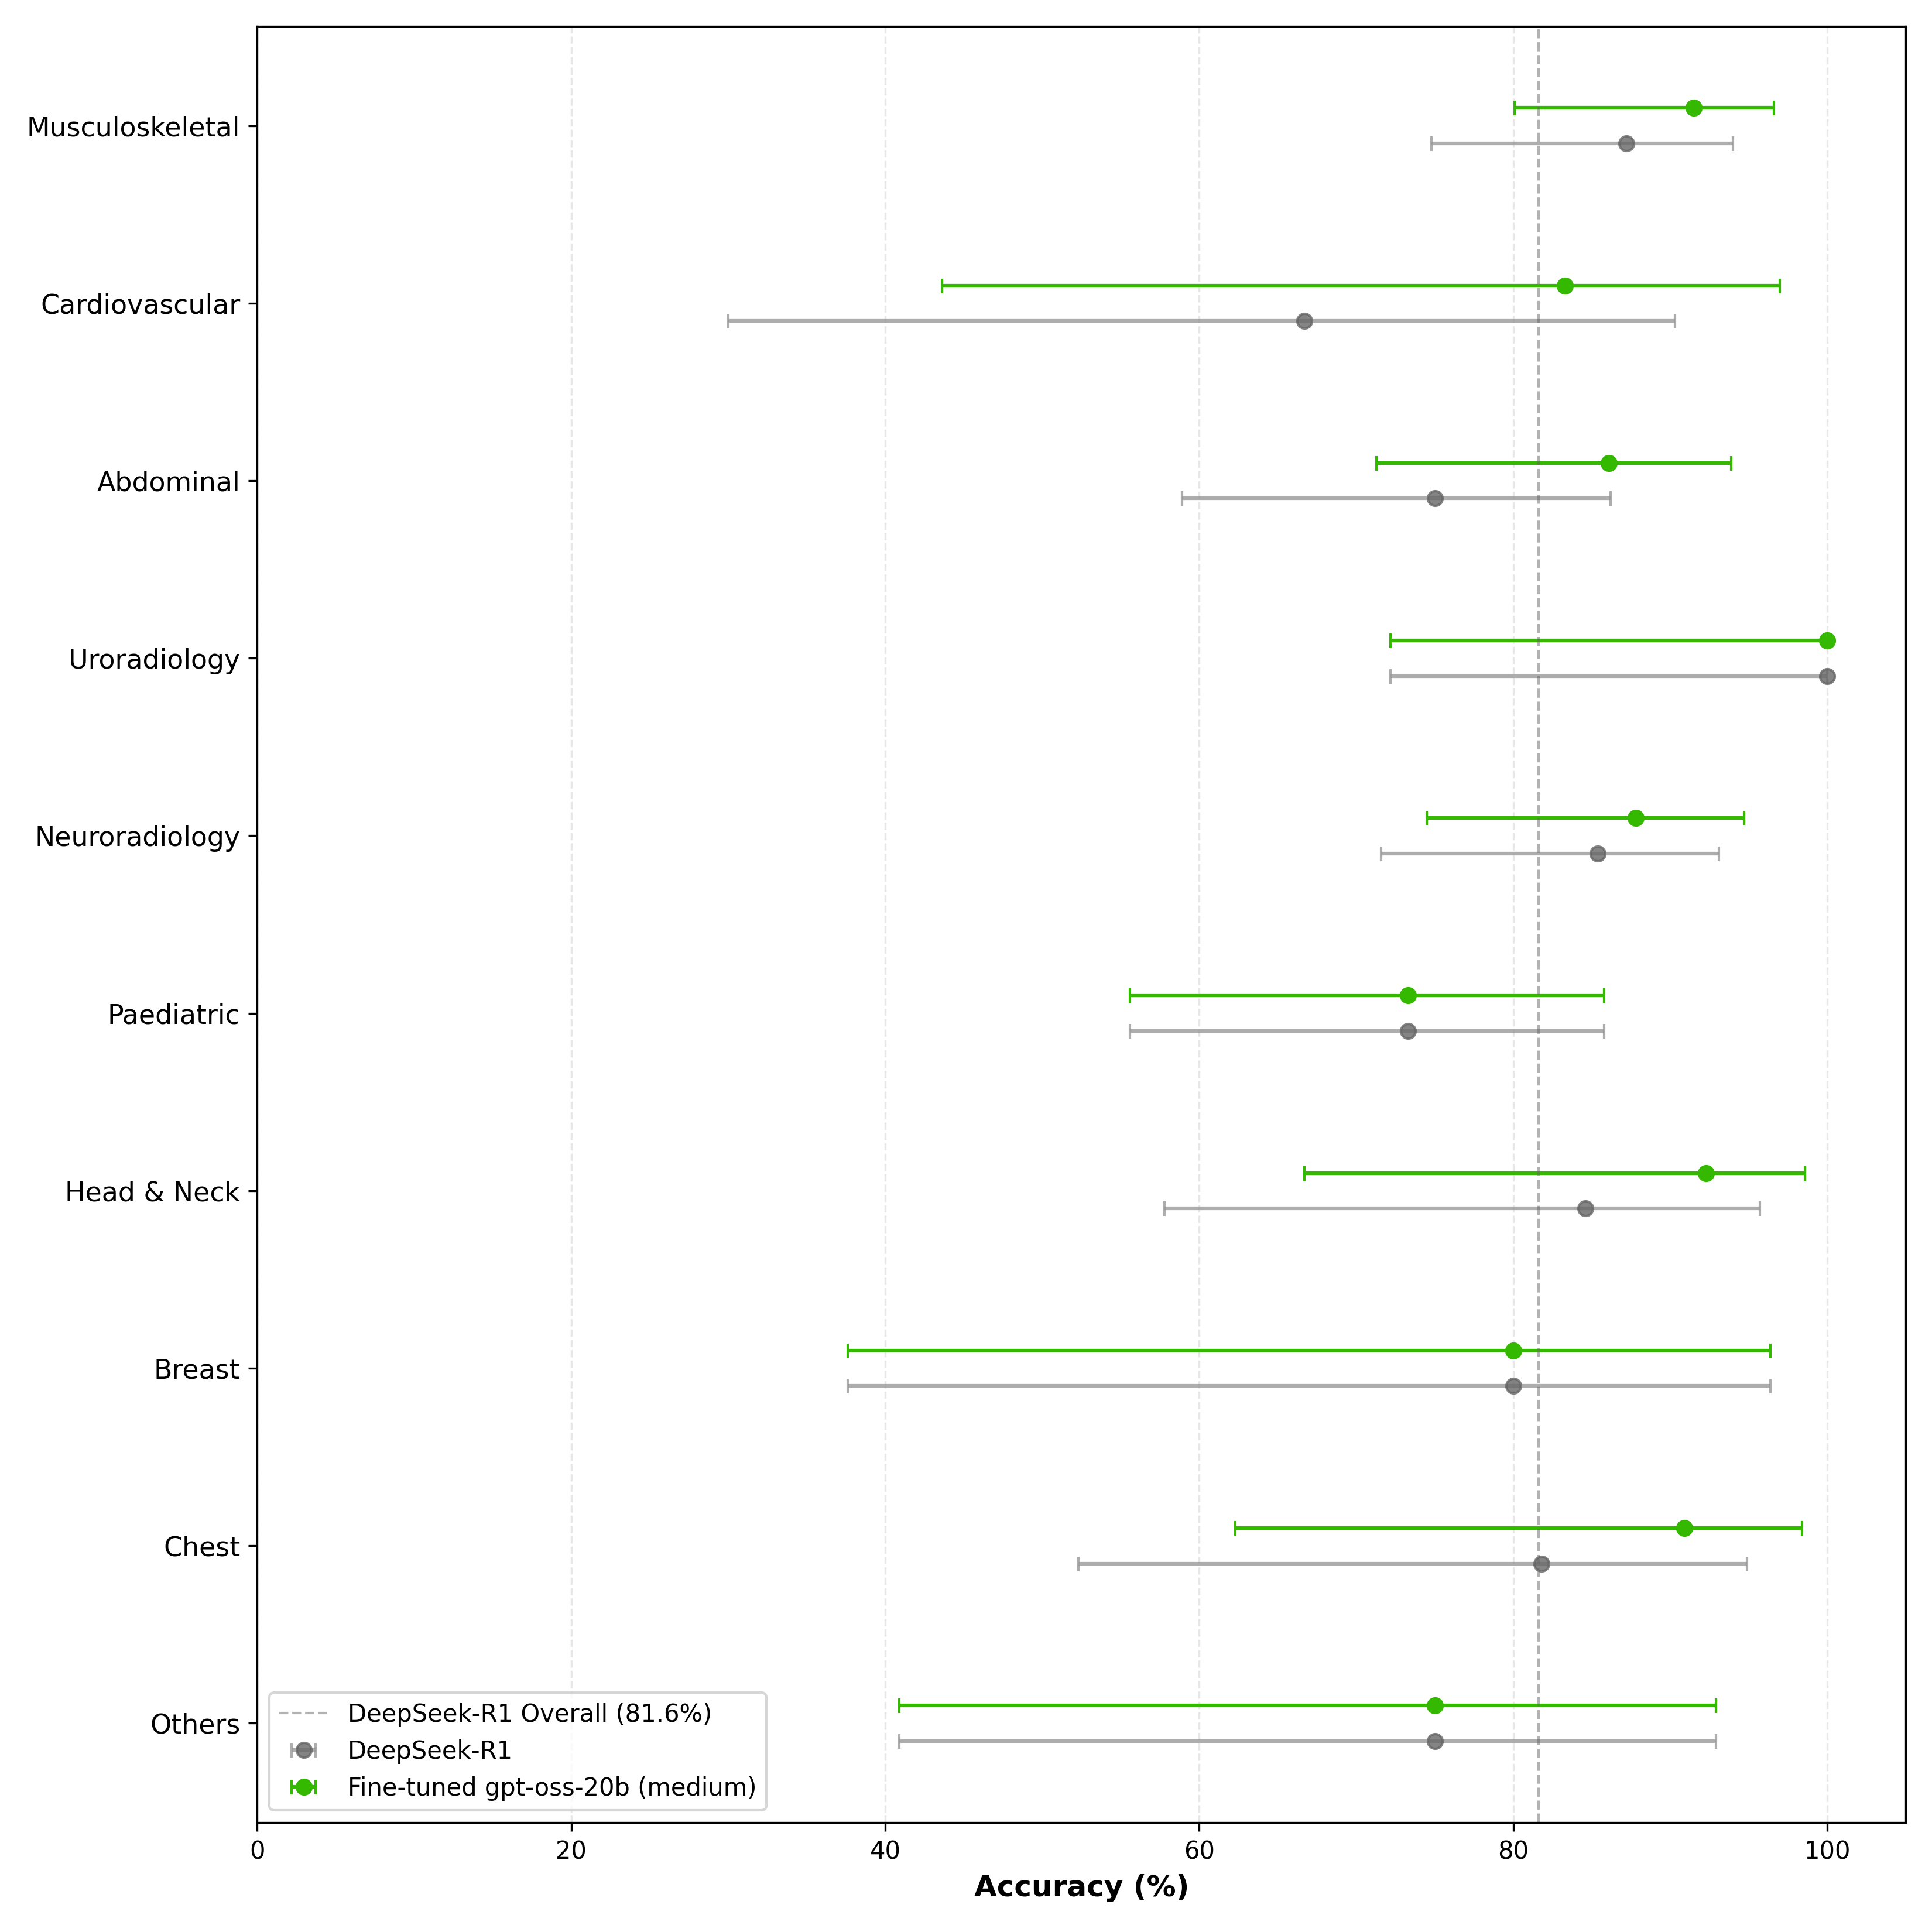
\includegraphics[width=\textwidth]{supp-imgs/manuscript_forest_plot_deepseek.png}
    \caption{\textbf{Parameter efficiency: Fine-tuned gpt-oss-20b model outperforms the 671B DeepSeek-R1.} 
    Comparative diagnostic accuracy of the fine-tuned gpt-oss-20b model (green) versus the open-source frontier DeepSeek-R1 (gray). Despite being significantly smaller, the fine-tuned on-device model achieves a higher overall micro-average accuracy (86.5\% vs 81.6\%) and demonstrates superior performance in 7 out of 10 anatomical subgroups. Error bars represent 95\% Wilson score intervals.}
    \vspace*{\fill}
\end{figure}

% --- Figure 2: o4-mini (Red vs Gray) ---
\clearpage
\begin{figure}[p]
    \centering
    \vspace*{\fill}
    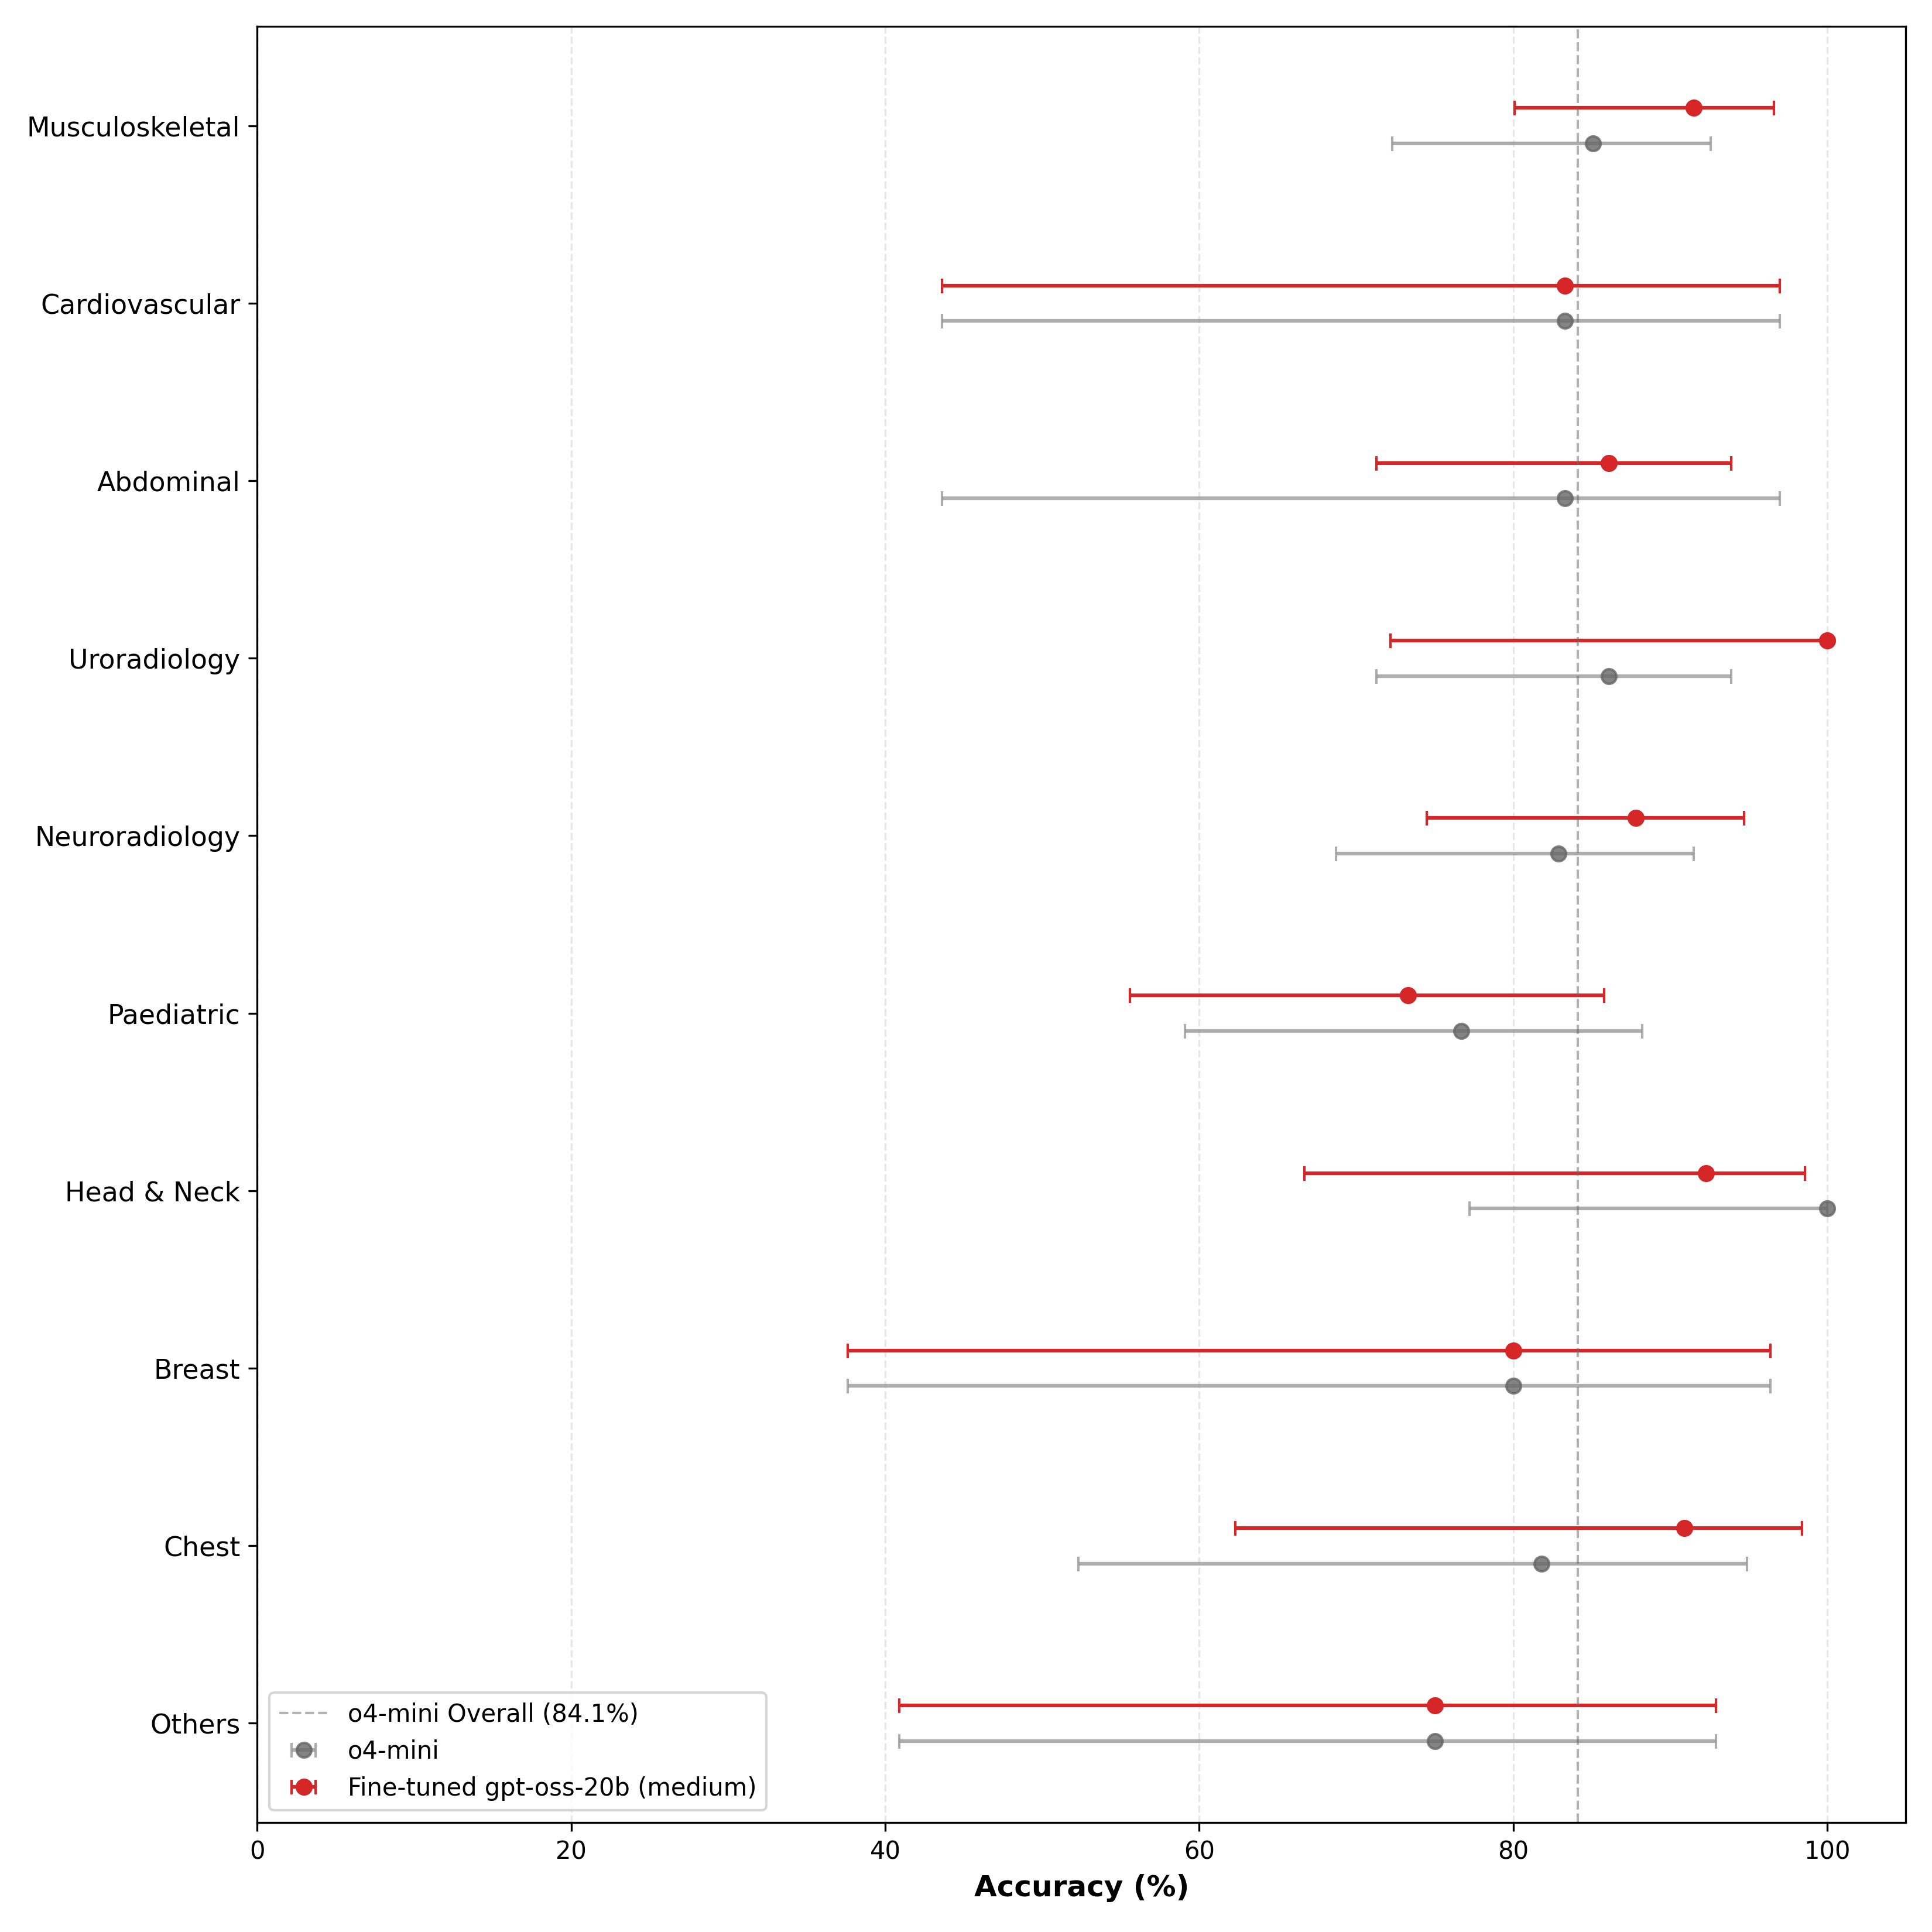
\includegraphics[width=\textwidth]{supp-imgs/manuscript_forest_plot_o4mini.png}
    \caption{\textbf{On-device versus cloud-based efficiency: Fine-tuned model surpasses o4-mini.} 
    Performance comparison between the fine-tuned gpt-oss-20b (red) and OpenAI's efficient proprietary model, o4-mini (gray). The on-device model demonstrates robust generalization, exceeding the cloud-based baseline in overall accuracy (86.5\% vs 84.1\%) and achieving competitive results across diverse radiological specialties. Vertical dashed lines indicate the overall micro-average accuracy for each model.}
    \vspace*{\fill}
\end{figure}

% --- Figure 3: GPT-5 (Blue vs Gray) ---
\clearpage
\begin{figure}[p]
    \centering
    \vspace*{\fill}
    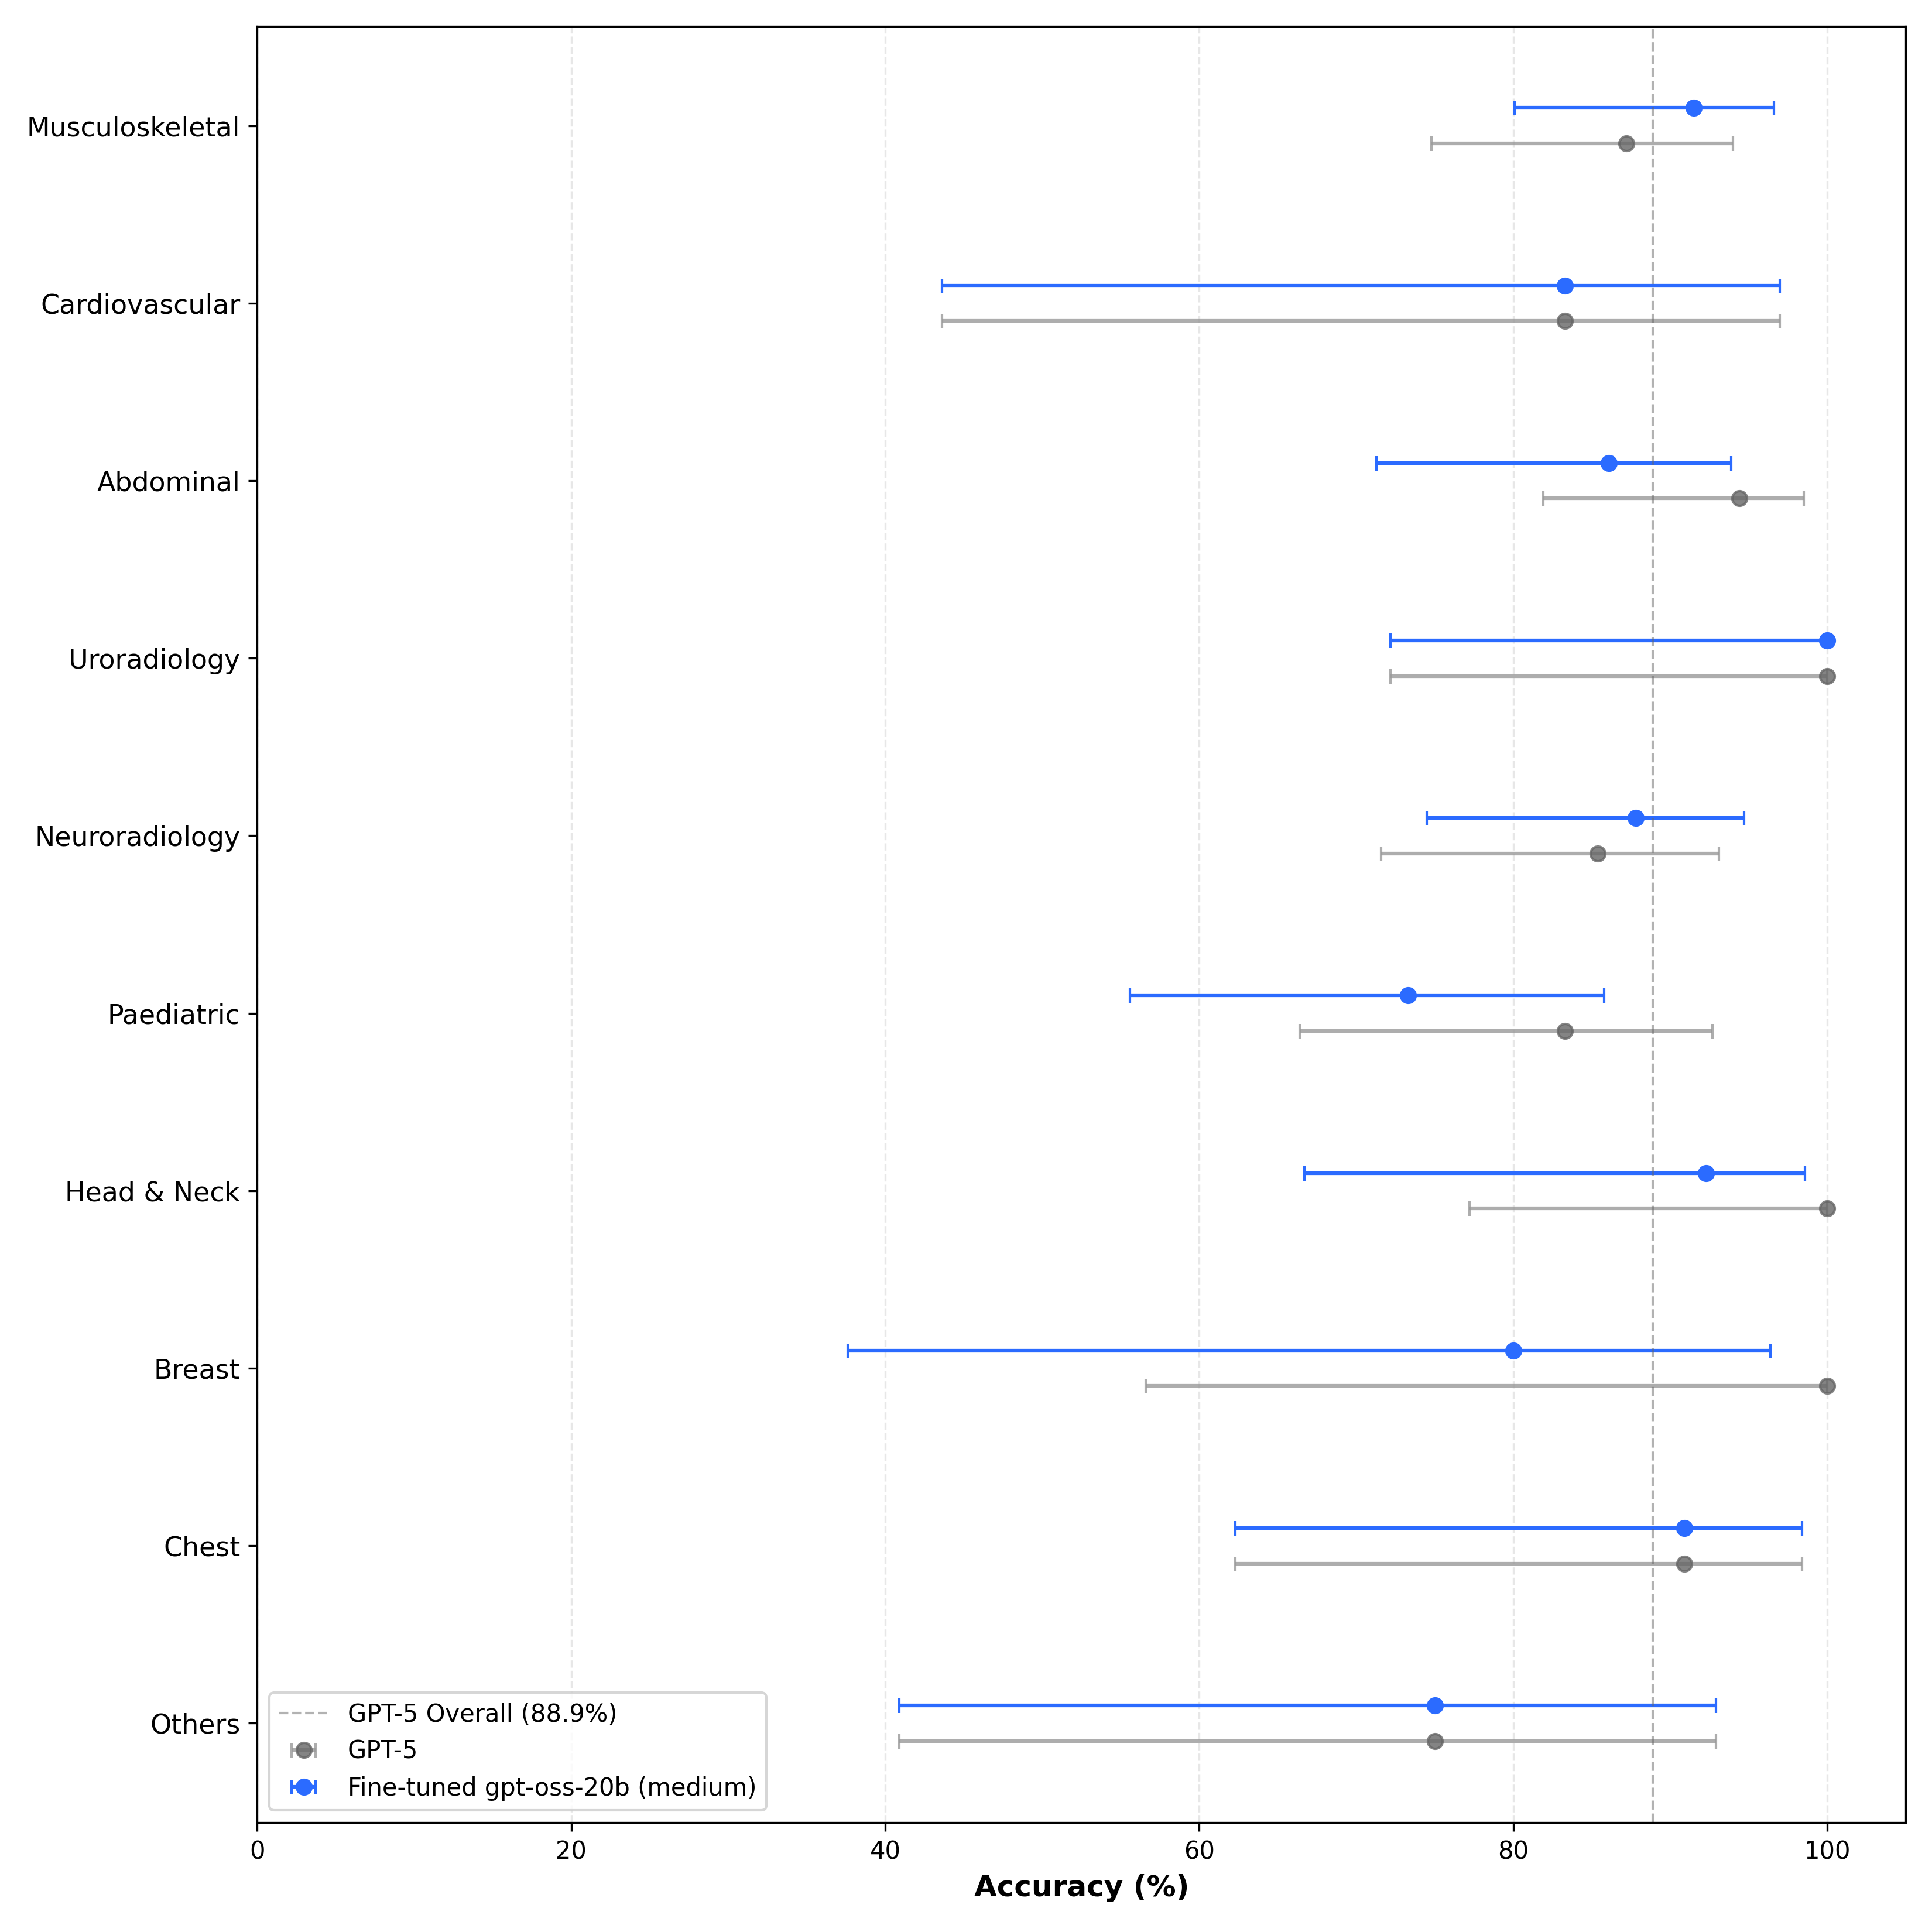
\includegraphics[width=\textwidth]{supp-imgs/manuscript_forest_plot_gpt5.png}
    \caption{\textbf{Approaching the frontier: On-device model demonstrates competitive performance with GPT-5.} 
    The forest plot illustrates the diagnostic accuracy of the fine-tuned gpt-oss-20b (blue) relative to the state-of-the-art GPT-5 (gray). While GPT-5 maintains a slight lead in overall accuracy (88.9\% vs 86.5\%), the confidence intervals overlap significantly across the majority of subgroups (e.g., Musculoskeletal, Abdominal, Neuroradiology), indicating statistical parity in these domains.}
    \vspace*{\fill}
\end{figure}
\clearpage

% Omar Case Studies
\section*{Case Studies}

% \subsection*{Fine-Tuned gptoss 20b Demonstrating Chain-of-Thought Reasoning with Systematic Elimination and Final Answer Selection}

% \section*{Case Studies: Fine-Tuned gptoss 20b Demonstrating Chain-of-Thought Reasoning with Systematic Elimination and Final Answer Selection}

The following case studies illustrate the chain-of-thought reasoning capabilities of gptoss 20b fine-tuned on the Eurorad radiology dataset. Each case demonstrates the model's systematic approach to differential diagnosis: (1) identifying core clinical-radiologic patterns, (2) mapping each differential to observed features, (3) systematically eliminating unlikely diagnoses, and (4) converging on a final answer with supporting rationale.


\vspace{1em}
% --- Case 1: Von Hippel-Lindau Syndrome (Before/After Fine-Tuning) ---
\begin{casebox}
    \textbf{Case Study 1: Von Hippel-Lindau Syndrome}

    \vspace{1em}
    \textbf{Case Presentation}
    
    \textbf{Clinical History:} A 41-year-old male presents with a history of microscopic haematuria, a palpable right flank mass, and recurrent headaches. A CT scan was performed, followed by a brain MRI to rule out tumoural pathology. The patient had no significant medical history.
    
    \vspace{1em}
    \textbf{Imaging Findings:} In the abdominal CT scan, multiple bilateral renal cystic lesions with septum formation were observed. The right kidney had multiple, irregular, heterogeneous lesions with significant enhancement post-contrast, and hypodense central areas related to necrosis, the biggest located in the superior pole. Similar characteristics were noted in the left kidney lesions. Also, multiple simple pancreatic cysts and splenic vein dilation were observed, along with pancreaticosplenic collaterals. There is a lesion in the splenic hilum that enhances and follows contrast in different phases, suggestive of a splenic hamartoma. The brain MRI revealed multiple heterogeneous lesions with a cystic and a solid component in the posterior fossa, showing avid and homogeneous enhancement of the solid portion, and causing vasogenic oedema and mass effect on the pons.
    
    \vspace{1em}
    \textbf{Differential diagnoses to consider:} Von Hippel-Lindau syndrome (VHL), Sporadic haemangioblastomas, Multiple endocrine neoplasia type 1 (MEN-1), Tuberous sclerosis complex (TSC), Polycystic kidney disease (PKD), Hereditary leiomyomatosis and renal cell cancer (HLRCC)
    
    \vspace{1em}
    \textbf{Ground Truth:} Von Hippel-Lindau syndrome (VHL)
    
    \vspace{1em}
    \hrule
    \vspace{1em}

    \textbf{Base Model Response (Before Fine-Tuning)}

    \vspace{1em}
    We need to consider the constellation: renal cystic lesions with septations, bilateral; pancreatic cysts; splenic hamartoma; brain hemangioblastomas. Also hematuria, flank mass. \textit{[Issue: Lists features but no systematic framework]}

    \vspace{0.5em}
    VHL is classic: bilateral clear cell RCC, hemangioblastomas of CNS, pancreatic cysts, renal cysts, etc. \textit{[Issue: Brief statement, no detailed reasoning]}

    \vspace{0.5em}
    MEN1: pituitary, parathyroid, pancreatic endocrine tumors, but not renal cysts or hemangioblastomas. \textit{[Issue: Superficial elimination - just "but not X"]}

    \vspace{0.5em}
    TSC: cortical tubers, subependymal nodules, renal angiomyolipomas, but not hemangioblastomas. \textit{[Issue: Lists features without explaining why they exclude diagnosis]}

    \vspace{0.5em}
    PKD: bilateral cystic kidneys, but not brain lesions. \textit{[Issue: One-sentence dismissal]}

    \vspace{0.5em}
    HLRCC: renal cell carcinoma (papillary type 2), cutaneous leiomyomas, uterine leiomyomas, but not brain hemangioblastomas. \textit{[Issue: No detailed analysis]}

    \vspace{0.5em}
    Thus VHL fits best. The presence of multiple bilateral renal cystic lesions with septations and enhancing lesions suggests clear cell RCC. The brain lesions are hemangioblastomas. Splenic hamartoma is also associated with VHL? \textit{[Issue: Shows uncertainty - questioning itself]} Splenic hamartoma is not classic but can be seen. Pancreatic cysts also seen. So VHL is the best. \textit{[Issue: Lacks confidence and systematic synthesis]}

    \vspace{1em}
    \noindent\textbf{Base Model Final Answer:} \colorbox{green!30}{Von Hippel-Lindau syndrome (VHL)} -- \textbf{CORRECT but with uncertain, superficial reasoning}

    \vspace{1em}
    \hrule
    \vspace{1em}

    \textbf{Fine-Tuned Model Response}

    \vspace{1em}
    \noindent\textbf{Step 1 -- Relate the clinical picture to the imaging}
    
    The patient is a 41-year-old man with microscopic haematuria, a palpable right-flank mass and recurrent headaches. \colorbox{yellow!30}{The flank mass corresponds to the enlarged, heterogeneous right kidney seen on CT}. The headaches are explained by the posterior-fossa lesions on brain MRI, which are cystic-solid, avidly enhancing and causing mass effect on the pons. The combination of renal cystic-solid lesions, pancreatic cysts, splenic vascular anomalies (splenic-vein dilation, pancreatic-splenic collaterals) and multiple posterior-fossa haemangioblastomas is highly suggestive of a hereditary tumour-spectrum disorder.
    
    \vspace{1em}
    \noindent\textbf{Step 2 -- Map findings to each differential}
    \vspace{1em}

    \renewcommand{\arraystretch}{1.5}
    \setlength{\tabcolsep}{10pt}
    {\footnotesize
    \begin{tabular}{|>{\raggedright\arraybackslash}p{2.5cm}|>{\raggedright\arraybackslash}p{4cm}|>{\raggedright\arraybackslash}p{3cm}|>{\raggedright\arraybackslash}p{2.5cm}|}
    \hline
    \textbf{Differential} & \textbf{Typical imaging/clinical hallmarks} & \textbf{Concordance with this case} & \textbf{Reason for exclusion} \\
    \hline
    \textbf{Von Hippel-Lindau (VHL)} & \textbf{Bilateral renal cystic-solid lesions (cystic-solid RCC), pancreatic cysts, splenic vascular malformations, multiple cerebellar/brain-stem haemangioblastomas, haematuria, flank mass, headaches.} & \textbf{All key features present; age fits (40-50 yr).} & \textbf{--} \\
    \hline
    Sporadic haemangioblastomas & Usually solitary, no systemic renal or pancreatic lesions. & Multiple haemangioblastomas present; renal and pancreatic findings are absent in sporadic disease. & Multiple haemangioblastomas with systemic findings exclude sporadic form. \\
    \hline
    MEN-1 & Pancreatic neuroendocrine tumours, parathyroid hyperplasia, pituitary adenomas; renal cysts are uncommon, haemangioblastomas are not typical. & Pancreatic cysts are simple, not neuroendocrine; no endocrine lesions reported; renal lesions are cystic-solid RCC, not typical MEN-1. & Absence of neuroendocrine tumours and endocrine dysfunction. \\
    \hline
    TSC & Multiple cortical tubers, subependymal nodules, renal angiomyolipomas (fat-dense), cardiac rhabdomyomas, retinal hamartomas. & No cortical tubers, no fat-dense renal lesions, no cardiac or retinal findings. & Pathognomonic TSC features (cortical tubers, angiomyolipomas) are absent. \\
    \hline
    PKD & Bilateral, large, non-enhancing cysts; no solid enhancing components; no pancreatic or splenic vascular lesions; no brain haemangioblastomas. & Renal lesions are cystic-solid with necrotic centres, not simple cysts; extra-renal lesions present. & Presence of solid enhancing components and extra-renal manifestations. \\
    \hline
    HLRCC & Renal cell carcinoma (often papillary type II) with aggressive behaviour; no pancreatic cysts or splenic vascular anomalies; no haemangioblastomas. & Renal lesions are cystic-solid but lack the classic papillary-type II morphology; extra-renal findings are absent in HLRCC. & Missing characteristic HLRCC features (aggressive papillary RCC, cutaneous leiomyomas). \\
    \hline
    \end{tabular}
    }
    
    \vspace{1em}
    \noindent\textbf{Step 3 -- Systematic elimination}
    \begin{itemize}[leftmargin=*, noitemsep, topsep=2pt]
        \item Sporadic haemangioblastomas are excluded because the patient has multiple CNS lesions accompanied by systemic renal and pancreatic manifestations, which are not seen in sporadic cases.
        \item MEN-1 is ruled out by the absence of neuroendocrine pancreatic tumours, parathyroid disease, or pituitary adenomas.
        \item TSC is eliminated by the absence of cortical tubers, subependymal nodules, and fat-dense angiomyolipomas.
        \item PKD is excluded because the renal lesions are cystic-solid with enhancing components and necrotic centres, not simple non-enhancing cysts.
        \item HLRCC is ruled out by the lack of aggressive papillary-type II RCC morphology and the presence of CNS haemangioblastomas, which are not part of HLRCC.
        \item \colorbox{yellow!30}{\textbf{Only VHL accounts for the complete constellation of findings}}: bilateral cystic-solid renal lesions, pancreatic cysts, splenic vascular anomalies, and multiple CNS haemangioblastomas.
    \end{itemize}
    
    \vspace{1em}
    \noindent\textbf{Step 4 -- Converge on the final diagnosis}
    
    The presence of bilateral cystic-solid renal lesions with necrotic centres, multiple simple pancreatic cysts, splenic vascular dilatation, and multiple posterior-fossa haemangioblastomas together with haematuria and a flank mass fits the classic VHL phenotype. \colorbox{yellow!30}{None of the other entities account for the full spectrum of findings}. The logical synthesis of clinical presentation and imaging demonstrates that the patient's findings are most consistent with Von Hippel-Lindau syndrome. Genetic confirmation (VHL gene mutation) would be the next step, followed by multidisciplinary surveillance for renal, pancreatic, splenic, and CNS manifestations.
    
    \vspace{1em}
    \noindent\textbf{Fine-Tuned Model Final Answer:} \colorbox{green!30}{\textbf{Von Hippel-Lindau syndrome (VHL)}} -- \textbf{CORRECT with systematic, confident reasoning}

    \vspace{1em}
    \hrule
    \vspace{1em}

    \textbf{Key Improvements from Fine-Tuning:}
    \begin{itemize}[leftmargin=*, noitemsep, topsep=2pt]
        \item \textbf{Structured framework:} Transformed unstructured list into systematic 4-step analysis with explicit clinical-imaging correlation
        \item \textbf{Comprehensive comparison:} Added detailed 6-syndrome table with concordance/discordance columns vs. brief text dismissals
        \item \textbf{Multi-system integration:} Step 1 explicitly synthesizes renal, pancreatic, splenic, and CNS findings into hereditary tumor syndrome pattern
        \item \textbf{Explicit elimination logic:} "Reason for exclusion" column with pathophysiologic justification vs. superficial "but not X" statements
        \item \textbf{Eliminated uncertainty:} Definitive statements about splenic findings vs. questioning ("Splenic hamartoma is also associated with VHL?")
        \item \textbf{Clinical confidence:} Comprehensive synthesis with next-step recommendations vs. tentative conclusion
    \end{itemize}
\end{casebox}


\vspace{1em}

% --- Case 2: Primary Cardiac Lymphoma (Before/After Fine-Tuning) ---
\begin{casebox}
    \textbf{Case Study 2: Primary Cardiac Lymphoma}

    \vspace{1em}
    \textbf{Case Presentation}
    
    \textbf{Clinical History:} An 81-year-old male with a history of paroxysmal atrial fibrillation presents to the emergency department with a one-week onset of orthopnoea and exertional dyspnoea. Laboratory tests demonstrate elevated troponins, the electrocardiogram reveals a third-degree atrioventricular block, and the echocardiogram shows right ventricular thickening and pericardial effusion.
    
    \vspace{1em}
    \textbf{Imaging Findings:} A PET-CT scan was carried out revealing a large hypermetabolic myocardial tissue. It extended through the right chambers and around the large vessels, sparing the left ventricle. Additionally, a hypermetabolic nodular image was identified at the left lung base. Therefore, a contrast-enhanced chest CT scan was performed. It confirmed the presence of an infiltrative hypodense mass in the myocardium. It involved the right atrium, right ventricle, interatrial septum, and atrioventricular groove. The mass caused mural thickening of the right cavities. A cuff encircled the right coronary artery along its course. A moderate pericardial effusion was also observed. Finally, the CT scan confirmed the solid nodule in the posterior segment of the left lower lobe. A CT-guided percutaneous biopsy of the lung nodule was made for histological examination.
    
    \vspace{1em}
    \textbf{Differential diagnoses to consider:} Angiosarcoma, IgG4-related disease, Primary cardiac lymphoma, Erdheim-Chester disease, Undifferentiated pleomorphic sarcoma
    
    \vspace{1em}
    \textbf{Ground Truth:} Primary cardiac lymphoma
    
    \vspace{1em}
    \hrule
    \vspace{1em}

    \textbf{Base Model Response (Before Fine-Tuning)}

    \vspace{1em}
    We need to reason step by step using only provided info. The case: 81-year-old male, paroxysmal atrial fibrillation, orthopnea, exertional dyspnea, elevated troponins, ECG shows third-degree AV block, echo shows right ventricular thickening and pericardial effusion. PET-CT shows large hypermetabolic myocardial tissue extending through right chambers and around large vessels, sparing left ventricle. Hypermetabolic nodular image at left lung base. Contrast CT confirms infiltrative hypodense mass in myocardium involving right atrium, right ventricle, interatrial septum, AV groove. Mural thickening of right cavities. Cuff around right coronary artery. Moderate pericardial effusion. Solid nodule in posterior segment left lower lobe. \textit{[Issue: Just lists findings without synthesis]}

    \vspace{0.5em}
    Let's analyze each:

    \vspace{0.5em}
    Angiosarcoma: Primary cardiac sarcoma, most common primary malignant tumor of heart. Usually involves right atrium, can extend to right ventricle, pericardial effusion, can cause arrhythmias, conduction block. PET hypermetabolic. Age: typically younger (median 40-50). But can occur in older. \textit{[Issue: Makes excuses instead of using age as exclusion criterion]} Lung metastasis possible. So fits. \textit{[Issue: Prematurely accepts this diagnosis]}

    \vspace{0.5em}
    IgG4-related disease: Infiltrative disease, can involve heart (IgG4-related pericarditis, myocarditis). Usually involves pericardium, can cause thickening, but not typically hypermetabolic mass on PET? Could show uptake. But IgG4 disease often involves multiple organs, but lung involvement can be nodules. However, IgG4 disease rarely presents as a large infiltrative mass in myocardium. Also would have elevated IgG4 levels, histology with IgG4 plasma cells. Not typical. \textit{[Issue: Rambling, uncertain reasoning]}

    \vspace{0.5em}
    Primary cardiac lymphoma: Rare, often involves right atrium, can cause conduction block, pericardial effusion, infiltration. PET hypermetabolic. Age: can be older. Lung involvement? Usually no lung nodules. But could metastasize to lung. But primary cardiac lymphoma often involves both atria and ventricles, but can be localized. Could present with AV block. So possible. \textit{[Issue: Doesn't recognize AV block as KEY feature for lymphoma]}

    \vspace{0.5em}
    Erdheim-Chester disease: Non-Langerhans cell histiocytosis, systemic infiltration, can involve heart (pericardial thickening, infiltration of myocardium). Usually involves both ventricles, but can involve right side. Also can involve lungs (nodules). Age: older adults. PET hypermetabolic. But typical features: symmetric osteosclerosis of long bones, retroperitoneal fibrosis, etc. Not mentioned. Also infiltration often involves both ventricles, not sparing left ventricle. So less likely. \textit{[Issue: Superficial elimination]}

    \vspace{0.5em}
    Undifferentiated pleomorphic sarcoma: A type of sarcoma, but not typical for heart. Could be primary cardiac sarcoma but usually angiosarcoma is most common. Undifferentiated pleomorphic sarcoma can be in heart but less common. Could present similarly. But the mass is hypermetabolic, infiltration of right chambers. Could be. \textit{[Issue: No real elimination logic]}

    \vspace{0.5em}
    We need to choose the most likely. The key features: right atrium/ventricle involvement, pericardial effusion, conduction block, hypermetabolic mass, lung nodule. Angiosarcoma is classic for right atrium, pericardial effusion, conduction block, metastasis to lung. \textit{[Issue: Misses that AV block is MORE classic for lymphoma]} Primary cardiac lymphoma also can present similarly. But which is more likely? Let's consider age: 81. Angiosarcoma usually younger. Primary cardiac lymphoma often in immunocompromised or older? Primary cardiac lymphoma can occur in older adults. But the presence of a lung nodule that was biopsied: likely metastasis. In angiosarcoma, lung metastases common. In primary cardiac lymphoma, metastasis to lung less common? Actually lymphoma can metastasize to lung. But the lung nodule is hypermetabolic. The biopsy would reveal histology. But we don't have histology results. \textit{[Issue: Circular reasoning without clear conclusion]}

    \vspace{0.5em}
    Angiosarcoma often shows infiltrative mass in right atrium, can extend to right ventricle, pericardial effusion, can encircle coronary arteries. The mass can be hypermetabolic. The left ventricle is spared. That fits. Primary cardiac lymphoma often involves both atria and ventricles, but can be localized. But the mass in this case is large, infiltrative, hypermetabolic, involving right atrium, right ventricle, interatrial septum, AV groove. That is typical for angiosarcoma. Also the presence of a lung nodule suggests metastasis. So angiosarcoma is likely. \textit{[Issue: Wrong conclusion - prioritized lung nodule over AV block]}

    \vspace{1em}
    \noindent\textbf{Base Model Final Answer:} \colorbox{red!30}{Angiosarcoma} -- \textbf{INCORRECT}

    \vspace{1em}
    \hrule
    \vspace{1em}

    \textbf{Fine-Tuned Model Response}

    \vspace{1em}
    \noindent\textbf{Step 1 -- Relate the clinical picture to the imaging}
    
    The patient is an elderly man with new-onset orthopnoea, exertional dyspnoea, a third-degree AV block, elevated troponin and a right-ventricular-predominant thickening on echo. \colorbox{yellow!30}{These findings point to a process that involves the right-sided myocardium, the conduction system (AV node)} and produces a pericardial effusion. The PET-CT shows a large, intensely FDG-avid mass that surrounds the right atrium, right ventricle, inter-atrial septum and the atrioventricular groove, sparing the left ventricle. A second hypermetabolic nodule is seen in the left lower-lobe lung, later confirmed as a metastatic lesion. Thus we have a right-sided cardiac infiltrative tumour with extra-cardiac metastasis.
    
    \vspace{1em}
    \noindent\textbf{Step 2 -- Map findings to each differential}
    \vspace{1em}

    \renewcommand{\arraystretch}{1.5}
    \setlength{\tabcolsep}{10pt}
    {\footnotesize
    \begin{tabular}{|>{\raggedright\arraybackslash}p{2.8cm}|>{\raggedright\arraybackslash}p{3.8cm}|>{\raggedright\arraybackslash}p{3.2cm}|>{\raggedright\arraybackslash}p{2.7cm}|}
    \hline
    \textbf{Differential} & \textbf{Typical imaging \& clinical features} & \textbf{Concordance with this case} & \textbf{Discordance} \\
    \hline
    \textbf{Primary cardiac lymphoma (PCL)} & \textbf{Usually involves right-sided chambers, encases AV node → AV block; often presents with pericardial effusion; may be FDG-avid; can metastasize to lung; left ventricle usually spared.} & \textbf{All three hallmarks present (right-sided infiltrate, AV block, pericardial effusion, lung metastasis, FDG avidity).} & \textbf{None.} \\
    \hline
    Angiosarcoma & Most common primary cardiac sarcoma; tends to involve right atrium, may cause hemopericardium, pericardial effusion; often shows heterogeneous enhancement, necrosis, and may invade coronary arteries. & Right-sided location and pericardial effusion fit. & Angiosarcoma usually shows a more heterogeneous, necrotic mass with prominent vascular channels; the PET-CT shows a uniformly hypermetabolic, well-circumscribed infiltrate, and the mass encircles the right coronary artery without obvious necrosis. Metastasis to lung is possible but less common than lymphoma. \\
    \hline
    IgG4-related disease & Can cause "tumefactive" cardiac lesions, but typically presents with systemic features (pancreatitis, retro-orbital disease), and imaging shows diffuse myocardial thickening rather than a discrete mass; PET may be mildly FDG-avid. & None of the systemic IgG4 manifestations are present. & Lack of extra-cardiac IgG4-related lesions and the aggressive, FDG-avid nature argue against it. \\
    \hline
    Erdheim-Chester disease & Bilateral symmetric osteosclerosis of long bones, pericardial thickening, retro-orbital pseudotumor; cardiac involvement is usually infiltrative but not as focal; PET may be positive. & No bone lesions or other classic sites. & Unlikely. \\
    \hline
    Undifferentiated pleomorphic sarcoma & Rare, often involves left ventricle, may be large, heterogeneous, necrotic, and can cause hemopericardium. & Right-sided location is atypical; mass is uniformly hypermetabolic without necrosis. & Unlikely. \\
    \hline
    \end{tabular}
    }
    
    \vspace{1em}
    \noindent\textbf{Step 3 -- Systematic elimination}
    \begin{itemize}[leftmargin=*, noitemsep, topsep=2pt]
        \item Angiosarcoma is less likely because the lesion is uniformly FDG-avid, lacks necrotic areas, and the patient's age (81) is above the typical 30-50 yr range.
        \item IgG4-related disease and Erdheim-Chester disease are excluded by the absence of systemic manifestations and characteristic extra-cardiac findings.
        \item Undifferentiated pleomorphic sarcoma is improbable given the right-sided predominance and lack of necrosis.
    \end{itemize}
    
    \vspace{1em}
    \noindent\textbf{Step 4 -- Converge on the most plausible diagnosis}
    
    The combination of (1) \colorbox{yellow!30}{right-sided cardiac infiltration with AV node encasement causing complete heart block}, (2) moderate pericardial effusion, (3) intense FDG uptake, (4) a solitary lung metastasis, and (5) the patient's age and clinical course, aligns perfectly with primary cardiac lymphoma. The subsequent CT-guided lung biopsy confirming metastatic lymphoma clinches the diagnosis.
    
    \vspace{1em}
    \noindent\textbf{Fine-Tuned Model Final Answer:} \colorbox{green!30}{\textbf{Primary cardiac lymphoma}} -- \textbf{CORRECT}

    \vspace{1em}
    \hrule
    \vspace{1em}

    \textbf{Key Improvements from Fine-Tuning:}
    \begin{itemize}[leftmargin=*, noitemsep, topsep=2pt]
        \item \textbf{Recognized key clinical feature:} Immediately identified AV node encasement causing third-degree AV block as pathognomonic for primary cardiac lymphoma
        \item \textbf{Systematic framework:} Transformed rambling analysis into structured 4-step approach with clear clinical synthesis
        \item \textbf{Detailed differential table:} Added comprehensive 5-entity comparison with concordance/discordance analysis vs. unstructured text
        \item \textbf{Proper age weighting:} Used patient age (81 years) to definitively exclude angiosarcoma (typical 30-50 yr) rather than making excuses
        \item \textbf{Imaging pattern recognition:} Identified "uniformly hypermetabolic, well-circumscribed" pattern as distinguishing from heterogeneous, necrotic angiosarcoma
        \item \textbf{Clinical correlation:} Step 4 synthesizes all findings (AV block + location + effusion + lung met + age) to converge on correct diagnosis
    \end{itemize}
\end{casebox}

\vspace{1em}

% --- Case 3: NICE Lesions (Before/After Fine-Tuning) ---
\begin{casebox}
    \textbf{Case Study 3: Non-Ischemic Cerebral Enhancing (NICE) Lesions}

    \vspace{1em}
    \textbf{Case Presentation}
    
    \textbf{Clinical History:} Five days after an uncomplicated embolisation of an asymptomatic, growing right middle cerebral artery (MCA) aneurysm, a 56-year-old woman comes to the ER due to headache, a seizure and fluctuant left upper extremity weakness and left campimetric defects. A Todd's paralysis is suspected, and the patient is admitted for a workup.
    
    \vspace{1em}
    \textbf{Imaging Findings:} Initially, a brain CT is performed, which shows no significant abnormalities apart from the embolisation material. Then a brain MRI is performed, including the following sequences: DWI, SWI, T2, FLAIR, 3D TOF and pre and post-gadolinium T1. The MRI discloses multiple round lesions varying in size in the right hemisphere. The lesions are spontaneously T1 hypointense and T2 hyperintense, the largest ones showing a small, central T2 hypointensity. Post-gadolinium enhancement is demonstrated in all the lesions. No restricted diffusion or susceptibility artefacts are present. Follow-up imaging after 6 months shows overall improvement with resolution of the enhancing foci. However, T2 hyperintensity is still present, and central punctate susceptibility artefacts have appeared, interpreted as microhaemorrhagic foci.
    
    \vspace{1em}
    \textbf{Differential diagnoses to consider:} Non-ischemic cerebral enhancing (NICE) lesions, Subacute cerebral infarcts, Cerebral microabscesses, Brain metastases
    
    \vspace{1em}
    \textbf{Ground Truth:} Non-ischemic cerebral enhancing (NICE) lesions
    
    \vspace{1em}
    \hrule
    \vspace{1em}

    \textbf{Base Model Response (Before Fine-Tuning)}

    \vspace{1em}
    We need to consider the imaging features: multiple round lesions, T1 hypointense, T2 hyperintense, central T2 hypointensity, post-gadolinium enhancement, no diffusion restriction, no susceptibility artifacts initially. After 6 months, resolution of enhancement, persistent T2 hyperintensity, central punctate susceptibility artifacts (microhemorrhages). \textit{[Issue: Lists features without prioritizing temporal context]}

    \vspace{0.5em}
    This suggests that the lesions were likely embolization-related changes: e.g., embolic microinfarcts? But no diffusion restriction. \textit{[Issue: Immediately questions own reasoning]} Subacute infarcts would show diffusion restriction early, then T2 hyperintensity, then resolution of enhancement? But subacute infarcts usually show restricted diffusion early, then T2 hyperintensity, then no enhancement. But here no diffusion restriction. \textit{[Issue: Circular reasoning]} Also multiple lesions after embolization could be due to embolic microinfarcts from procedure. But the lesions are enhancing, which is not typical for infarcts. However, early subacute infarcts can show enhancement due to breakdown of BBB. But they usually show diffusion restriction early. But maybe small lesions might not show diffusion restriction? \textit{[Issue: Making excuses for contradictory evidence instead of using it to exclude]} But central T2 hypointensity suggests hemorrhagic component? But no susceptibility artifacts initially. After 6 months, microhemorrhages appear. Could be due to microinfarcts with hemorrhagic transformation? But microhemorrhages appear later. \textit{[Issue: Continued circular reasoning]}

    \vspace{0.5em}
    Alternatively, could be cerebral microabscesses? They would show diffusion restriction, rim enhancement, central T2 hyperintensity. But no diffusion restriction. So unlikely.

    \vspace{0.5em}
    Brain metastases: multiple enhancing lesions, T1 hypointense, T2 hyperintense, central T2 hypointensity? Usually metastases have ring enhancement, central necrosis, sometimes hemorrhage. But metastases would show diffusion restriction? Not necessarily. But metastases would not spontaneously resolve after 6 months unless treated. Also patient had no known primary cancer. So less likely.

    \vspace{0.5em}
    Non-ischemic cerebral enhancing (NICE) lesions: This is a broad category. \textit{[Issue: Dismisses correct answer as "too broad"]} Could include inflammatory lesions, demyelinating lesions, etc. But the context of embolization suggests procedure-related changes. Could be "post-embolization changes" like "cerebral embolic infarcts" or "cerebral microinfarcts" that enhance due to BBB breakdown. The resolution of enhancement over 6 months fits with healing of infarcts. The persistent T2 hyperintensity indicates gliosis or chronic changes. The microhemorrhages appear later due to microinfarcts with hemorrhagic transformation. \textit{[Issue: Talks around NICE but doesn't recognize it as specific diagnosis]}

    \vspace{0.5em}
    Thus the most likely is Subacute cerebral infarcts. \textit{[Issue: Wrong conclusion - failed to use absence of DWI restriction as definitive exclusion criterion]}

    \vspace{1em}
    \noindent\textbf{Base Model Final Answer:} \colorbox{red!30}{Subacute cerebral infarcts} -- \textbf{INCORRECT}

    \vspace{1em}
    \hrule
    \vspace{1em}

    \textbf{Fine-Tuned Model Response}

    \vspace{1em}
    \noindent\textbf{Step 1 -- Relate the clinical picture to the imaging problem}
    
    The patient had a recent endovascular embolisation of a right MCA aneurysm. Five days later she develops a new headache, a focal seizure and transient left-sided weakness with visual field loss. This post-intervention presentation with focal neurological deficits \colorbox{yellow!30}{immediately suggests a complication} rather than a primary neoplasm or infection. The transient weakness is classic for Todd's paralysis, which is a post-ictal phenomenon that can mimic a new infarct.
    
    \vspace{1em}
    \noindent\textbf{Step 2 -- Describe the MRI pattern and map to differentials}
    
    \textbf{MRI Pattern:}
    \begin{itemize}[leftmargin=*, noitemsep, topsep=2pt]
        \item Multiple round foci confined to the right cerebral hemisphere (the side of the intervention).
        \item Spontaneous T1-hypointensity, T2-hyperintensity, with a small central T2-hypointense core.
        \item Uniform, homogeneous post-gadolinium enhancement in all lesions.
        \item No diffusion restriction on DWI, no blooming on SWI at the initial scan.
        \item Follow-up (6 mo) shows resolution of enhancement, persistent T2 hyperintensity, and new tiny susceptibility foci (micro-haemorrhages).
    \end{itemize}
    This pattern is characteristic of NICE lesions: they are multiple, well-circumscribed, enhance avidly, lack diffusion restriction, and evolve to a non-enhancing T2-hyperintense state with occasional micro-bleeds.
    
    \vspace{1em}
    \renewcommand{\arraystretch}{1.5}
    \setlength{\tabcolsep}{10pt}
    {\footnotesize
    \begin{tabular}{|>{\raggedright\arraybackslash}p{2.8cm}|>{\raggedright\arraybackslash}p{4.2cm}|>{\raggedright\arraybackslash}p{5.0cm}|}
    \hline
    \textbf{Differential} & \textbf{Expected imaging features} & \textbf{Concordance/discordance with case} \\
    \hline
    \textbf{NICE (post-embolisation)} & \textbf{Multiple, round, enhancing lesions confined to the ipsilateral hemisphere; no diffusion restriction; may show central T2 hypointensity; evolution to non-enhancing T2 hyperintensity with micro-bleeds.} & \textbf{All criteria met: multiple right-hemisphere lesions, homogeneous enhancement, no DWI restriction, central T2 core, evolution pattern.} \\
    \hline
    Subacute cerebral infarcts & Usually wedge-shaped, follow vascular territories; diffusion restriction present in the acute/subacute phase; may show blooming on SWI due to haemorrhagic conversion; enhancement is often peripheral and delayed. & Lesions are round, not territorial; no diffusion restriction; no SWI blooming initially; enhancement is uniform, not peripheral. \\
    \hline
    Cerebral microabscesses & Often solitary or few, ring-enhancing with central diffusion restriction; may have surrounding oedema; SWI may show central susceptibility. & Multiple lesions, no diffusion restriction, no oedema, uniform rather than ring enhancement. \\
    \hline
    Brain metastases & Usually multiple, often peripherally located, may have surrounding oedema, variable enhancement (often heterogeneous), and frequent susceptibility artefacts from haemorrhage. & Lesions are confined to one hemisphere, lack surrounding oedema, enhancement is homogeneous, and initial SWI is negative. \\
    \hline
    \end{tabular}
    }
    
    \vspace{1em}
    \noindent\textbf{Step 3 -- Systematic elimination}
    \begin{itemize}[leftmargin=*, noitemsep, topsep=2pt]
        \item Subacute infarcts are excluded by the absence of diffusion restriction and the non-territorial, round morphology. \colorbox{yellow!30}{Acute ischemic lesions would show restricted diffusion}, which is not present here.
        \item Microabscesses are unlikely because there is no diffusion restriction, no oedema, and the enhancement is not ring-like. Abscesses typically show a hyperintense DWI core.
        \item Metastases are improbable given the unilateral distribution, lack of perilesional oedema, and the temporal relationship to a recent endovascular procedure. The patient also has no known primary malignancy.
        \item The combination of a recent aneurysm embolisation, unilateral multiple enhancing lesions without diffusion restriction, central T2 hypointensity, and the characteristic evolution (resolution of enhancement, persistence of T2 hyperintensity, and later micro-bleeds) fits the classic profile of NICE lesions.
    \end{itemize}
    
    \vspace{1em}
    \noindent\textbf{Step 4 -- Converge on the final diagnosis}
    
    \colorbox{yellow!30}{The temporal relationship to endovascular intervention is the key clinical clue}. The combination of multiple ipsilateral round enhancing lesions without diffusion restriction, the presence of central T2 hypointensity, and the characteristic 6-month evolution (resolution of enhancement with persistent T2 signal and development of micro-haemorrhages) is pathognomonic for non-ischemic cerebral enhancing (NICE) lesions. Recognizing this pattern prevents unnecessary invasive workup and guides appropriate follow-up imaging.
    
    \noindent\textbf{Fine-Tuned Model Final Answer:} \colorbox{green!30}{\textbf{Non-ischemic cerebral enhancing (NICE) lesions}} -- \textbf{CORRECT}

    \hrule
    \vspace{1em}

    \textbf{Key Improvements from Fine-Tuning:}
    \begin{itemize}[leftmargin=*, noitemsep, topsep=2pt]
        \item \textbf{Recognized temporal context:} Immediately identified "5 days post-embolization" as key diagnostic clue for procedural complication (NICE lesions)
        \item \textbf{Used absence of DWI restriction definitively:} Applied lack of diffusion restriction to systematically exclude infarcts rather than making excuses
        \item \textbf{Eliminated circular reasoning:} Replaced "But maybe..." contradictions with clear exclusion logic based on imaging features
        \item \textbf{Recognized NICE as specific diagnosis:} Understood NICE lesions as established post-procedural entity, not just "broad category"
        \item \textbf{Applied evolution pattern:} Used 6-month follow-up (resolution of enhancement → persistent T2 → microbleeds) as pathognomonic feature
        \item \textbf{Systematic framework:} Transformed rambling analysis into structured 4-step approach with clear MRI pattern description and differential table
    \end{itemize}
\end{casebox}
%Omare end of case studies 





% \newpage
% \bibliographystyle{IEEEtran}
% \bibliography{supp}

\end{document}


